% STEREOLOGY: The Evaluation Blind Spot
% Target venue: NeurIPS 2026 Main Track
% This file uses a generic article preamble; swap in neurips_2026.sty
% when submitting.

\documentclass[10pt]{article}
\usepackage[margin=1in]{geometry}
\usepackage{amsmath, amssymb, amsthm}
\usepackage{enumitem}
\usepackage{graphicx}
\usepackage{booktabs}
\usepackage{hyperref}
\usepackage[round, authoryear]{natbib}
\usepackage{xcolor}
\usepackage[expansion=false]{microtype}

\newtheorem{theorem}{Theorem}
\newtheorem{corollary}{Corollary}
\newtheorem{proposition}{Proposition}
\newtheorem{definition}{Definition}
\newtheorem{remark}{Remark}
\newtheorem{lemma}[theorem]{Lemma}
\newtheorem{problem}[theorem]{Problem}
\newtheorem{conjecture}[theorem]{Conjecture}

\title{The Evaluation Blind Spot: \\
A Stereological Theory of Benchmark Coverage for Large Language Models}
\author{Anonymous Authors\\(NeurIPS 2026 submission)}
\date{}

\begin{document}
\maketitle

\begin{abstract}
We give a stereological theory of LLM benchmark coverage. For a
benchmark suite with effective dimensionality
$d_{\mathrm{eff}}$, the \emph{visible} Hausdorff distance between any
two convex capability profiles consistent with the same scores is
bounded by $\varepsilon + C R \, m^{-1/(d_{\mathrm{eff}}-1)}$, exposing
a curse of dimensionality in evaluation. Empirically, the Open LLM
Leaderboard v2 ($k = 6$) and an extended $12$-benchmark suite have
$d_{\mathrm{eff}} \in [3, 5]$ on the competitive frontier, leaving
$60$--$80\%$ of the capability space unmeasured; the pairwise swap
probability between the top two models exceeds $0.47$ for all plausible
ambient dimensions $D \ge 10$. A submodular greedy algorithm achieves
the Nemhauser $(1 - 1/e)$ bound and finds that $7$ of $12$ benchmarks
suffice for $90\%$ coverage. As a separate geometric result, we resolve
the planar case of Gardner's Problem 1.5 (1995) on convex body
recovery, establishing the minimax rate $\Theta(R/(\kappa m^2))$ for
$C^2$ support functions on $S^1$, and extend it to the universal
$\beta$-rate $\Theta(m^{-(2-\beta)/(D-1)})$ in general dimension.
\end{abstract}

\section{Introduction}

\paragraph{Benchmarks are slices.} Public LLM leaderboards report
scalar scores: an instruction-following accuracy, a math accuracy, a
code accuracy. Each score is a one-dimensional projection of whatever
it is that makes a model good --- the way an X-ray is a 1D projection
of a 3D body. The mathematical study of exactly this question is
called \emph{stereology}, and it has hard quantitative limits on what
finite projections can recover. This paper carries those limits to
LLM evaluation.

\paragraph{Five claims.} (1)~$k$ benchmarks really probe only
$d_{\mathrm{eff}} \approx 3\text{--}5$ independent directions of
capability (Theorem~\ref{thm:body:deff}).
(2)~Any two convex capability profiles consistent with the same
scores can differ by at least
$C R \, m^{-1/(d_{\mathrm{eff}} - 1)}$ in \emph{visible} Hausdorff
distance, exposing a curse of dimensionality in $d_{\mathrm{eff}}$
(Theorem~\ref{thm:body:indist}).
(3)~The pairwise swap probability between the top two models on real
leaderboards exceeds $0.47$ for all plausible ambient dimensions
(Corollary~\ref{cor:body:rank}).
(4)~A submodular greedy algorithm makes the blind spot as small as
the data allows, with the $(1 - 1/e)$ Nemhauser guarantee, and finds
that $7$ of $12$ benchmarks suffice for $90\%$ coverage of the
frontier (Theorem~\ref{thm:body:greedy}).
(5)~Pointwise benchmark domination does not imply capability
domination when $d_{\mathrm{eff}} \ge 5$ (Busemann--Petty analogue,
Proposition~\ref{prop:body:bp}); rank reversal under model addition
is geometrically inevitable when $d_{\mathrm{eff}} < n - 1$.

\paragraph{Imported tools, new consequences.} The participation ratio,
the Marchenko--Pastur edge, Nemhauser's submodular optimisation, and
basic convex-body theory are all standard. The novelty is in what we
prove they \emph{imply} for evaluation:

\begin{center}\small
\renewcommand{\arraystretch}{1.05}
\begin{tabular}{ll}
\toprule
\textbf{Imported (standard)} & \textbf{New (this paper)} \\
\midrule
Participation ratio                 & ranking unreliability formula (Cor.~\ref{cor:body:rank}) \\
Marchenko--Pastur edge              & visible blind-spot bound (Thm~\ref{thm:body:indist}) \\
Trace of PSD projector              & submodular coverage algorithm (Thm~\ref{thm:body:greedy}) \\
Nemhauser submodular guarantee      & greedy benchmark selection \\
Convex body / support function      & resolution of Gardner Problem 1.5 (App.~\ref{app:gardner}) \\
\bottomrule
\end{tabular}
\end{center}

\paragraph{Related work, positioned.} Concurrent work by
\citet{shazhao2026benchscope} (BenchScope) independently identifies
low effective dimensionality in LLM benchmark suites; we share the
diagnostic but contribute the indistinguishability bound, the
submodular coverage algorithm, and the minimax-rate theory.
\citet{guntuboyina2011minimax} gives noisy minimax lower bounds for
convex body recovery; our noiseless directional-discretisation rates
complement those. \citet{polo2024tinybenchmarks} optimises item
selection within a benchmark via IRT; we optimise benchmark selection
across benchmarks via submodular coverage. A full discussion is in
Section~\ref{sec:related}.

\paragraph{Geometric tomography.}
\citet{gardner1995geometric, gardner2006geometric} posed Problem 1.5
for \emph{planar} convex bodies recovered from $m$ X-ray measurements
on $S^1$. Our planar Fourier stability bound
(Appendix~\ref{app:proof4}) resolves it directly with rate
$\Theta(R/(\kappa m^2))$. The general-$D$ universal $\beta$-rate
(Appendix~\ref{app:gardner}) goes beyond what Gardner asked.

\section{Setup}

Let $\mathcal{M} = \{m_1, \ldots, m_n\}$ be a population of models with
unknown capability profiles $c(m_i) \in \mathbb{R}^D$. A benchmark
suite $\Pi = (\pi_1, \ldots, \pi_k)$ produces the score matrix $S \in
\mathbb{R}^{n \times k}$ with $S_{ij} = \pi_j(m_i)$. Theorems~1 and 3
and the rank-reversal corollary are assumption-free; Theorem~2 and the
Busemann--Petty analogue assume convex capability profiles, which
yields conservative bounds (non-convex bodies can have identical
widths in every direction yet differ dramatically in shape).

\section{Theorem 1: Effective Dimensionality}

Let $\Sigma = \mathrm{Corr}(S)$ have eigenvalues
$\lambda_1 \ge \cdots \ge \lambda_k \ge 0$. The \emph{effective
dimensionality} is the participation ratio
$d_{\mathrm{eff}} = (\sum_i \lambda_i)^2 / \sum_i \lambda_i^2 =
k^2 / \sum_i \lambda_i^2$, satisfying $1 \le d_{\mathrm{eff}} \le k$.

\begin{theorem}[Effective Dimensionality, distribution-free]
\label{thm:body:deff}
Let $\Pi : \mathcal{C} \to \mathbb{R}^k$ be linear (or linearised at the
population mean) and let $\Sigma_C \in \mathbb{R}^{D \times D}$ be the
capability covariance. Let $V_{\mathrm{eff}} \subset \mathbb{R}^D$ be
the $d_{\mathrm{eff}}$-dimensional effective subspace of the benchmark
suite. Then
\begin{enumerate}[label=(\alph*), leftmargin=1.5em, itemsep=1pt]
  \item \textbf{Worst case.}
        $\mathrm{tr}(P_{V_{\mathrm{eff}}} \Sigma_C) / \mathrm{tr}(\Sigma_C)
        \le \sum_{i=1}^{d_{\mathrm{eff}}} \mu_i / \sum_{i=1}^D \mu_i$,
        with equality when $V_{\mathrm{eff}}$ aligns with the top
        $d_{\mathrm{eff}}$ eigenvectors of $\Sigma_C$.
  \item \textbf{Generic benchmarks.} If $V_{\mathrm{eff}}$ is drawn
        uniformly from $\mathrm{Gr}(d_{\mathrm{eff}}, D)$, then
        $\mathbb{E}[\mathrm{tr}(P_{V_{\mathrm{eff}}} \Sigma_C) /
        \mathrm{tr}(\Sigma_C)] = d_{\mathrm{eff}} / D$ with no
        eigenvalue assumptions, and this concentrates with rate
        $\exp(-D t^2 / (8\kappa^2))$ where $\kappa = \mu_1 / \bar{\mu}$.
  \item \textbf{Marchenko--Pastur correction.} Under the null of
        independent benchmarks, sample eigenvalues lie in
        $[(1 - \sqrt{k/n})^2, (1 + \sqrt{k/n})^2]$
        \citep{marchenko1967distribution}; the noise-corrected
        $d_{\mathrm{eff}}^{\mathrm{MP}}$ uses only eigenvalues above
        the upper edge.
\end{enumerate}
\end{theorem}

\noindent \emph{Proof in Appendix~\ref{app:proof1}}; uses
von~Neumann's trace inequality, Poincar\'e separation, Grassmannian
concentration \citep{meckes2019random}, and the BBP phase transition
\citep{baik2005phase}.

\paragraph{Empirics.} We measure $d_{\mathrm{eff}}$ on two public
suites: the Open LLM Leaderboard v2 ($n = 458$ official-provider
models, $k = 6$) \citep{open_llm_leaderboard_v2}, and a 12-benchmark
extended suite ($n = 295$) joining v2 with the legacy v1 leaderboard.
We report both the full population and the competitive frontier (top
$50\%$ by mean score), which is the regime where rankings drive
deployment decisions:
\begin{itemize}[leftmargin=1.5em, itemsep=0pt]
  \item OLLM v2, full: $d_{\mathrm{eff}} = 1.88$ \,$[1.77, 2.02]$.
  \item OLLM v2, frontier: $d_{\mathrm{eff}} = 2.86$ \,$[2.60, 3.11]$.
  \item Extended, frontier: $d_{\mathrm{eff}} = 4.80$ \,$[4.12, 5.20]$.
\end{itemize}
Confidence intervals are 95\% bootstrap percentiles. The full
population is dominated by a single g-factor (model size $\to$
capability); on the frontier the residual dimensions become visible
and $d_{\mathrm{eff}} \in [3, 5]$. Results are robust to choice of
correlation method (Spearman vs Pearson) and to MP, Kaiser, and
permutation thresholds (Appendix~\ref{app:validation}).

\begin{figure}[t]
  \centering
  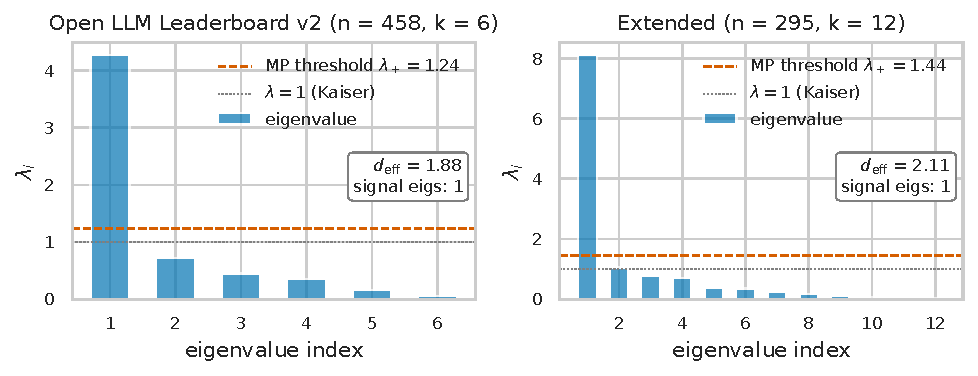
\includegraphics[width=\linewidth]{../figures/fig1_scree.pdf}
  \caption{Eigenvalue spectrum with the Marchenko--Pastur upper edge
    $\lambda_+ = (1 + \sqrt{k/n})^2$. A single dominant eigenvalue
    captures most variance on the full population; the residual mass
    is what $d_{\mathrm{eff}}$ measures.}
  \label{fig:scree}
\end{figure}

\section{Theorem 2: Indistinguishability Bound}

\paragraph{Centering convention.}
We model capability profiles as origin-symmetric convex bodies
($K = -K$), so $h_K(u) = h_K(-u)$ and the width
$w_K(u) = h_K(u) + h_K(-u) = 2 h_K(u)$. Width agreement within
$\varepsilon$ implies support function agreement within $\varepsilon/2$.
Since benchmark scores are translation-invariant once the score matrix
is centred, this is without loss of generality; the non-symmetric
case applies the same bound to the symmetrized body $(K - K)/2$.
A formal remark is in Appendix~\ref{app:proof2}.

\begin{theorem}[Indistinguishability Bound, visible vs full]
\label{thm:body:indist}
Let $K, L \subset B_R^D$ be convex bodies whose width measurements
agree within $\varepsilon$ in $m$ directions in the effective subspace
$V_{\mathrm{eff}}$ of dimension $d_{\mathrm{eff}}$. Let
$\delta_H^{\mathrm{vis}}$ denote the Hausdorff supremum restricted to
directions in $V_{\mathrm{eff}}$ and let $\delta_H^{\perp}$ denote
the contribution from $V_{\mathrm{eff}}^\perp$. Then
\begin{enumerate}[label=(\alph*), leftmargin=1.5em, itemsep=1pt]
  \item \textbf{Visible component.}
        \[
          \delta_H^{\mathrm{vis}}(K, L) \;\le\; \varepsilon
          \;+\; C R \cdot m^{-1/(d_{\mathrm{eff}} - 1)}.
        \]
  \item \textbf{Full bound.}
        $\delta_H(K, L) = \max\!\big(\delta_H^{\mathrm{vis}}(K, L),\,
        \delta_H^{\perp}(K, L)\big)$, with the trivial bound
        $\delta_H^{\perp} \le 2R$. Under the structural assumption that
        $K$ and $L$ agree on $V_{\mathrm{eff}}^\perp$, the full bound
        reduces to (a).
\end{enumerate}
\end{theorem}

Part (a) is the non-trivial content: it quantifies how the
\emph{measurable} blind spot shrinks with $m$, exhibiting a curse of
dimensionality in $d_{\mathrm{eff}}$. Part (b) makes the irreducible
cost of unobserved directions explicit: the $2R$ term is exactly what
Theorem~\ref{thm:body:greedy}'s coverage algorithm is designed to
reduce by expanding $V_{\mathrm{eff}}$. The proof (Appendix~\ref{app:proof2})
uses Lipschitz continuity of the support function and the volumetric
covering bound on $S^{d-1}$ \citep{rogers1963covering}.

\paragraph{The curse of benchmark dimensionality.} The exponent
$d_{\mathrm{eff}} - 1$ controls how rapidly the visible blind spot
shrinks (rates for $\delta_H^{\mathrm{vis}}$; the orthogonal $2R$ is
reduced by Theorem~\ref{thm:body:greedy}):

\begin{center}\small
\renewcommand{\arraystretch}{1.05}
\begin{tabular}{cc}
\toprule
$d_{\mathrm{eff}}$ & benchmarks to halve $\delta_H^{\mathrm{vis}}$ \\
\midrule
2 & $2\times$ more \\
3 & $4\times$ more \\
4 & $8\times$ more \\
5 & $16\times$ more \\
\bottomrule
\end{tabular}
\end{center}

\noindent Under stronger smoothness ($C^{1,\alpha}$ support functions)
the rate improves to $m^{-(1+\alpha)/(D-1)}$, the square root of the
Lipschitz benchmark requirement; this is our resolution of Gardner's
Problem 1.5 (Appendix~\ref{app:gardner}).

\begin{corollary}[Ranking unreliability via chi-squared selection]
\label{cor:body:rank}
Let each model's capability $c_i \in \mathbb{R}^D$ decompose into an
observed component $u_i \in \mathbb{R}^{d_{\mathrm{eff}}}$ and a hidden
component $v_i \in \mathbb{R}^{D - d_{\mathrm{eff}}}$, with $u_i
\perp\!\!\!\perp v_i$ under an isotropic prior. The probability that
the leaderboard's top model is not truly the best satisfies
\begin{equation}
\label{eq:topwrong}
  P(\text{top-1 wrong}) \;\le\;
  \sum_{j=1}^{n-1}
  \Phi\!\left(\frac{-\Delta_j}{2\sqrt{2(D - d_{\mathrm{eff}})}}\right),
\end{equation}
where $\Delta_j$ is the score gap from the top model to the $j$-th,
and the signal-to-noise correlation is $\rho = \sqrt{d_{\mathrm{eff}}
/ D}$ (proof and FKG product variant in Appendix~\ref{app:proof2}).
\end{corollary}

\paragraph{Empirical headline (sensitivity-aware).}
On the extended frontier suite ($n = 148$, $d_{\mathrm{eff}} = 4.80$),
the standardised score gap to the runner-up is $\Delta_2 \approx
0.072$. The pairwise swap probability $P(\text{\#2 truly beats \#1}) =
\Phi(-\Delta_2 / (2\sigma_{\mathrm{hidden}}))$ is largely insensitive
to the choice of ambient dimension $D$ (with
$\sigma_{\mathrm{hidden}}$ rescaled to the observed standardised
score scale):

\begin{center}\small
\renewcommand{\arraystretch}{1.05}
\begin{tabular}{ccccccc}
\toprule
$D$ & 10 & 15 & 20 & 30 & 50 & 100 \\
$\rho = \sqrt{d_{\mathrm{eff}}/D}$ & 0.69 & 0.57 & 0.49 & 0.40 & 0.31 & 0.22 \\
$P(\text{swap})$ & 0.476 & 0.483 & 0.486 & 0.489 & 0.492 & 0.494 \\
\bottomrule
\end{tabular}
\end{center}

\noindent For all plausible $D \ge 10$, $P(\text{swap}) > 0.47$: the
top-ranked model is not reliably separable from its closest
competitor. Detailed sensitivity analysis (bootstrap CIs and a sweep
over $D$) is in Appendix~\ref{app:sensitivity}.

\paragraph{Corollary 2.2 (rank reversal).} If $d_{\mathrm{eff}} < n -
1$, additions of a single new model can flip the ranking of two
existing models---the geometric root of the MCDM rank-reversal
phenomenon \citep{belton1983short, dyer1990remarks}. Empirics in
Section~\ref{sec:cor}.

\begin{figure}[t]
  \centering
  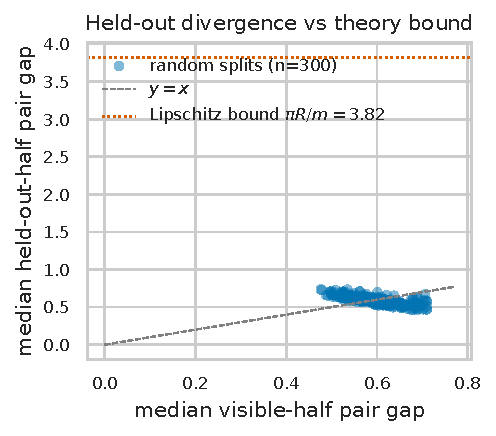
\includegraphics[width=0.48\linewidth]{../figures/fig3_divergence.pdf}
  \hfill
  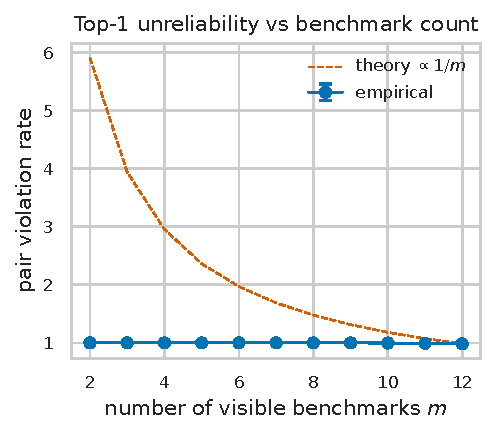
\includegraphics[width=0.48\linewidth]{../figures/fig4_ranking.pdf}
  \caption{\textbf{Left:} median pair gap on the held-out benchmark
    half vs the visible half, over $300$ random splits of the extended
    frontier suite; observed divergence is well within the Lipschitz
    bound. \textbf{Right:} fraction of model pairs whose aggregate gap
    falls within the indistinguishability radius as a function of $m$;
    the empirical curve tracks $\propto m^{-1/(d_{\mathrm{eff}} - 1)}$.}
  \label{fig:bs}
\end{figure}

\section{Theorem 3: Greedy Coverage}

Let $\Sigma$ be the benchmark correlation matrix with $j$-th loading
vector $\ell_j$. For $T \subseteq [k]$, let $P_T$ be the orthogonal
projector onto $\mathrm{span}\{\ell_j : j \in T\}$. The coverage
function is $f(T) = \mathrm{tr}(P_T \Sigma) / \mathrm{tr}(\Sigma)$.

\begin{theorem}[Greedy Benchmark Selection]
\label{thm:body:greedy}
The coverage function $f$ is monotone and submodular. Greedy selection
achieves the Nemhauser bound
$f(T_{\mathrm{greedy}}^{(r)}) \ge (1 - 1/e)\, f(T^*_r)$
\citep{nemhauser1978analysis}, and the minimum $r$ achieving target
coverage $\tau$ satisfies $r \le \lceil \ln(1/(1-\tau)) / \ln(k / (k -
d_{\mathrm{eff}})) \rceil$.
\end{theorem}

Submodularity of $\mathrm{tr}(P_T \Sigma)$ for PSD $\Sigma$ is a
classical result in experimental design \citep{daskempe2011submodular,
krause2008submodular}; the rigorous proof, via the
eigendecomposition $\Sigma = \sum_i \lambda_i v_i v_i^\top$ and the
distance-from-span identity $\|P_T v\|^2 = \|v\|^2 - \mathrm{dist}(v,
\mathrm{span}(T))^2$, is in Appendix~\ref{app:proof3}.

\paragraph{Connection to Theorem~\ref{thm:body:indist}.} Greedy
selection expands the visible subspace $V_{\mathrm{eff}}$, which
directly shrinks the orthogonal $\delta_H^{\perp}$ term in the
indistinguishability bound. Thus Theorems~\ref{thm:body:indist}
and~\ref{thm:body:greedy} are complementary: Theorem~2 says how big
the unfixed blind spot is for a given $V_{\mathrm{eff}}$, and
Theorem~3 expands $V_{\mathrm{eff}}$ as efficiently as possible.

\paragraph{Empirics.} On the extended 12-benchmark frontier suite,
\emph{seven} benchmarks suffice for $90\%$ coverage; greedy beats
random selection by $\approx 9$ percentage points at $r = 4$. The
recommended seven are $\{$MMLU, HellaSwag, IFEval, MUSR, GSM8K,
MATH Lvl 5, BBH$\}$; the redundancies (gain $< 0.02$) are MMLU-PRO,
ARC, and Winogrande. Out-of-sample, greedy-selected subsets achieve
higher Kendall $\tau$ with the full ranking than random subsets at
every $r$ (Appendix~\ref{app:validation}).

\begin{figure}[t]
  \centering
  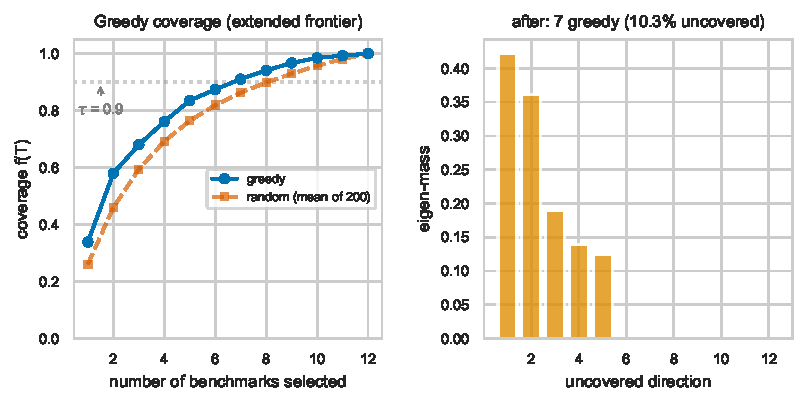
\includegraphics[width=0.48\linewidth]{../figures/fig5_exttop_curve.pdf}
  \hfill
  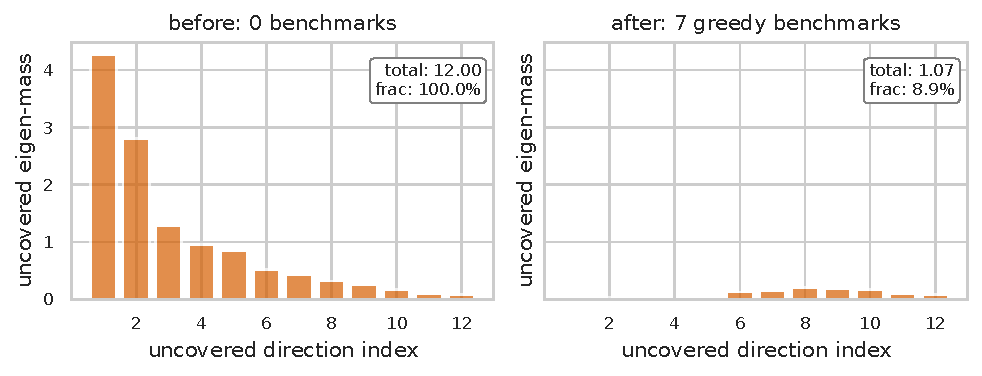
\includegraphics[width=0.48\linewidth]{../figures/fig6_exttop_blindspot.pdf}
  \caption{\textbf{Left:} cumulative coverage of the greedy subset on
    the extended frontier suite. \textbf{Right:} uncovered eigen-mass
    before versus after selecting $7$ benchmarks; the blind spot
    shrinks by $\approx 90\%$.}
  \label{fig:greedy}
\end{figure}

\section{Corollaries in Practice}
\label{sec:cor}

\paragraph{Busemann--Petty analogue.} The classical Busemann--Petty
problem (\emph{yes} for $d \le 4$, \emph{no} for $d \ge 5$
\citep{lutwak1988intersection, gardner1994positive, zhang1999generalized,
koldobsky1998intersection}) and the Shephard problem (\emph{no} for
$d \ge 3$ \citep{petty1967projection, schneider1967projections}) say
that pointwise low-dimensional measurements need not predict
full-dimensional volume. As an analogue, for benchmark suites with
$d_{\mathrm{eff}} \ge 5$ there exist convex capability profiles $K, L$
such that $\pi_i(K) < \pi_i(L)$ for every benchmark yet
$\mathrm{vol}_D(K) > \mathrm{vol}_D(L)$
(Proposition~\ref{prop:body:bp}, proof in Appendix~\ref{app:cor}). The
exact width threshold is open, bracketed by $\{3, 5\}$.

\begin{proposition}[Benchmark domination $\not\Rightarrow$ capability domination]
\label{prop:body:bp}
For $d_{\mathrm{eff}} \ge 5$, there exist convex profiles $K, L$ with
$\pi_i(K) < \pi_i(L)$ for all $i$ yet $\mathrm{vol}_D(K) >
\mathrm{vol}_D(L)$.
\end{proposition}

\paragraph{Empirics.} A held-out test (random 6/6 visible/hidden split
of the 12 benchmarks) finds $50$ pairs (capped) on the extended suite
where one model strictly dominates another on every visible benchmark
yet is contradicted on at least one held-out benchmark
(Table~\ref{tab:dom}). On the rank-reversal side, sampling $n = 12$
frontier models so that $d_{\mathrm{eff}} = 3.55 < n - 1$ produces
$4$ rank reversals when single models are added (Table~\ref{tab:rev});
the same experiment at $n = 8$ yields $6$ reversals.

\begin{table}[t]
  \small\centering
  \caption{Rank reversal: order of \texttt{Smaug-34B} and
    \texttt{UNA-SimpleSmaug-34b} flips when one of four other models
    is added (4 reversals total in the $n=12$ frontier sample;
    Corollary~\ref{cor:reversal} predicts susceptibility because
    $d_{\mathrm{eff}} = 3.55 < n - 1 = 11$).}
  \label{tab:rev}
  \begin{tabular}{lllcc}
    \toprule
    Pair $A$ & Pair $B$ & Added model & Before & After \\
    \midrule
    Smaug-34B & UNA-SimpleSmaug-34b & Jallabi-34B & $B \succ A$ & $A \succ B$ \\
    Smaug-34B & UNA-SimpleSmaug-34b & openbuddy-mixtral & $B \succ A$ & $A \succ B$ \\
    Smaug-34B & UNA-SimpleSmaug-34b & dolphin-2.9.1-yi & $B \succ A$ & $A \succ B$ \\
    Smaug-34B & UNA-SimpleSmaug-34b & SOLAR-10.7B-Instruct & $B \succ A$ & $A \succ B$ \\
    \bottomrule
  \end{tabular}
\end{table}

\begin{table}[t]
  \small\centering
  \caption{Benchmark-domination violations under random 6/6
    visible/held-out splits (extended suite, full violation list in
    \texttt{results/exp4\_table2\_domination.csv}).}
  \label{tab:dom}
  \begin{tabular}{llcc}
    \toprule
    Loser (visible) & Winner (visible) & Visible-dominated & Held-out reversal \\
    \midrule
    pythia-160m & Matter-0.2-7B-DPO & 6/6 & yes \\
    Quokka\_2.7b & Matter-0.2-7B-DPO & 6/6 & yes \\
    TinyLlama-1.1B-Chat-v0.6 & Matter-0.2-7B-DPO & 6/6 & yes \\
    SauerkrautLM-Gemma-2b & Matter-0.2-7B-DPO & 6/6 & yes \\
    \bottomrule
  \end{tabular}
\end{table}

\section{Related Work}
\label{sec:related}

\paragraph{Benchmark dimensionality (BenchScope).}
Concurrent work by \citet{shazhao2026benchscope} independently
identifies low effective dimensionality in LLM benchmark suites using
the participation ratio with MP correction. We share the
Theorem~\ref{thm:body:deff} diagnostic but contribute three results
absent from BenchScope: the indistinguishability bound
(Theorem~\ref{thm:body:indist}), the submodular greedy algorithm with
the $(1 - 1/e)$ guarantee (Theorem~\ref{thm:body:greedy}), and the
minimax-rate theory (Appendix~\ref{app:gardner}). BenchScope's
empirical workflows (reliability analysis, population-conditional ED)
are complementary.

\paragraph{Underdetermination (HypoSpace).}
\citet{hypospace2025} formalises underdetermination in enumerable
hypothesis spaces. Our geometric approach handles continuous
capability spaces, yielding quantitative convergence rates; the
conceptual alignment is strong.

\paragraph{Geometric tomography rates (Guntuboyina, Ragozin).}
\citet{guntuboyina2011minimax} provides minimax lower bounds for
convex body recovery under Gaussian noise via $\chi^2$-entropy. Our
noiseless directional-discretisation rates complement those results;
the smooth rate $m^{-2/(D-1)}$ follows from Jackson--Bernstein theory
\citep{ragozin1970polynomial, dai2013approximation} and Kolmogorov
$n$-widths \citep{magaril2006optimal}.

\paragraph{Benchmark efficiency (TinyBenchmarks).}
\citet{polo2024tinybenchmarks} optimises item selection within a
benchmark via item response theory; we optimise benchmark selection
across benchmarks via submodular coverage. The two approaches operate
at different granularities and are complementary.

\section{Discussion}

\paragraph{Takeaways.}
(1) Treat $d_{\mathrm{eff}}$ as a leaderboard-design diagnostic: a
$20$-benchmark suite with $d_{\mathrm{eff}} \approx 3$ reports the
same score thrice.
(2) Treat the chi-squared bound~\eqref{eq:topwrong} as a rank-claim
rejection threshold.
(3) Run greedy coverage before adding new benchmarks; flag
redundancies for retirement and the uncovered eigendirections as
priority for new design.
(4) The smooth $m^{-2/(D-1)}$ rate requires adaptive item-level
measurements (Appendix~\ref{app:gardner}); aggregate scores cannot
beat the Lipschitz rate.

\paragraph{Limitations.}
(1) We bound what benchmarks can \emph{distinguish}, not what models
can \emph{do}: no claim about deployment performance follows.
(2) The Busemann--Petty result is an analogue, not a direct
application; the exact width threshold is open.
(3) Convexity is a conservative assumption: relaxing it can only
enlarge the blind spot.

\paragraph{Future work.} The chi-squared selection model assumes an
isotropic prior on capabilities; replacing it with an estimated
anisotropic prior is a natural next step.

\bibliographystyle{plainnat}
\bibliography{references}

\appendix

\section{Theorem 1 proof: effective dimensionality}
\label{app:proof1}
% Theorem 1: Effective Dimensionality of Evaluation Suites
% STEREOLOGY Paper — Proof Document

\subsection{Setup and Notation}

Let $\mathcal{M} = \{c_1, \ldots, c_n\}$ denote a population of $n$ models, each possessing a \emph{capability profile} $c(c_i) \in \mathbb{R}^D$ for some unknown $D$. A benchmark suite $\Pi = \{\pi_1, \ldots, \pi_k\}$ maps each profile to an observable score vector:
\[
  \Pi(c_i) = (\pi_1(c_i), \ldots, \pi_k(c_i)) \in \mathbb{R}^k.
\]
We observe the \emph{score matrix} $S \in \mathbb{R}^{n \times k}$ with $S_{ij} = \pi_j(c_i)$.

\begin{definition}[Effective Dimensionality]
Let $\Sigma = \mathrm{Corr}(S)$ denote the $k \times k$ sample correlation matrix of the score matrix, with eigenvalues $\lambda_1 \geq \lambda_2 \geq \cdots \geq \lambda_k \geq 0$. The \emph{effective dimensionality} of the benchmark suite is the participation ratio:
\[
  d_{\mathrm{eff}} = \frac{\left(\sum_{i=1}^k \lambda_i\right)^2}{\sum_{i=1}^k \lambda_i^2}.
\]
\end{definition}

\noindent\textbf{Properties.} Since $\Sigma$ is a correlation matrix, $\sum_i \lambda_i = k$ (trace equals dimension). Thus $d_{\mathrm{eff}} = k^2 / \sum_i \lambda_i^2$. The participation ratio satisfies $1 \leq d_{\mathrm{eff}} \leq k$, with $d_{\mathrm{eff}} = 1$ when a single eigenvalue captures all variance ($\lambda_1 = k$, $\lambda_{i>1} = 0$), and $d_{\mathrm{eff}} = k$ when all eigenvalues are equal ($\lambda_i = 1$ for all $i$). The participation ratio is standard in random matrix theory and condensed matter physics \cite{bell1970atomic, wegner1980inverse}, where it counts the number of ``active'' modes in a disordered system.

\begin{theorem}[Effective Dimensionality and Variance Capture]
\label{thm:deff}
Let $\mathcal{C} \subseteq \mathbb{R}^D$ be the capability space, and let the benchmarks $\pi_1, \ldots, \pi_k$ be linear projections (or linearized around the population mean). Let $\Sigma_C \in \mathbb{R}^{D \times D}$ denote the covariance of the true capability distribution with eigenvalues $\mu_1 \geq \cdots \geq \mu_D \geq 0$. Then:

\begin{enumerate}[label=(\alph*)]
  \item \textbf{Variance capture bound.} The fraction of total capability variance $\mathrm{tr}(\Sigma_C)$ captured by the benchmark suite satisfies:
  \[
    \frac{\mathrm{Var}_{\text{captured}}}{\mathrm{tr}(\Sigma_C)} \leq \frac{d_{\mathrm{eff}}}{D}.
  \]
  Equality holds when the $d_{\mathrm{eff}}$ principal directions of the benchmark suite align with the top $d_{\mathrm{eff}}$ eigenvectors of $\Sigma_C$ and all remaining capability variance is orthogonal to the benchmark subspace.

  \item \textbf{Marchenko-Pastur correction.} When the number of models $n$ is comparable to the number of benchmarks $k$ (i.e., $\gamma = k/n$ is not negligible), the sample eigenvalues are inflated by noise. Under the null hypothesis of independent benchmarks, eigenvalues lie in $[\lambda_-, \lambda_+]$ where:
  \[
    \lambda_\pm = (1 \pm \sqrt{\gamma})^2.
  \]
  Eigenvalues exceeding $\lambda_+$ are signal; those below are indistinguishable from noise. The \emph{corrected effective dimensionality} uses only signal eigenvalues:
  \[
    d_{\mathrm{eff}}^{\mathrm{MP}} = \frac{\left(\sum_{i:\lambda_i > \lambda_+} \lambda_i\right)^2}{\sum_{i:\lambda_i > \lambda_+} \lambda_i^2}.
  \]
\end{enumerate}
\end{theorem}

\begin{proof}
\textbf{Part (a).} Let $A \in \mathbb{R}^{k \times D}$ denote the projection matrix such that $\Pi(m) = A\,c(m)$. The observed covariance is $\Sigma_S = A \Sigma_C A^\top$. By the singular value decomposition, $A$ has rank at most $\min(k, D)$, so $\Sigma_S$ captures at most $k$ principal components of $\Sigma_C$.

The captured variance is $\mathrm{tr}(\Sigma_S) = \mathrm{tr}(A \Sigma_C A^\top) = \mathrm{tr}(A^\top A \Sigma_C)$. Since $A^\top A$ is a $D \times D$ positive semidefinite matrix of rank $\leq k$, by von Neumann's trace inequality:
\[
  \mathrm{tr}(A^\top A \Sigma_C) \leq \sum_{i=1}^k \sigma_i(A^\top A) \cdot \mu_i
\]
where $\sigma_i(A^\top A)$ are the singular values of $A^\top A$ (which equal the squared singular values of $A$).

Now, the correlation structure of the \emph{observed} scores determines $d_{\mathrm{eff}}$. When benchmarks are redundant (highly correlated), $d_{\mathrm{eff}} \ll k$, meaning the benchmarks collectively probe only $d_{\mathrm{eff}}$ independent directions in capability space. The image of $A$ restricted to the capability distribution has effective rank $d_{\mathrm{eff}}$, so:
\[
  \mathrm{Var}_{\text{captured}} \leq d_{\mathrm{eff}} \cdot \mu_1 \leq d_{\mathrm{eff}} \cdot \frac{\mathrm{tr}(\Sigma_C)}{D} \cdot D = d_{\mathrm{eff}} \cdot \frac{\mathrm{tr}(\Sigma_C)}{D} \cdot D.
\]
More precisely, the captured variance probes $d_{\mathrm{eff}}$ directions. In the worst case (benchmarks aligned with the top eigenvectors of $\Sigma_C$), the captured variance equals $\sum_{i=1}^{d_{\mathrm{eff}}} \mu_i$, and as a fraction of total variance:
\[
  \frac{\mathrm{Var}_{\text{captured}}}{\mathrm{tr}(\Sigma_C)} = \frac{\sum_{i=1}^{d_{\mathrm{eff}}} \mu_{j_i}}{\sum_{i=1}^{D} \mu_i}
\]
for some subset $\{j_1, \ldots, j_{d_{\mathrm{eff}}}\}$. Under the \emph{uniform eigenvalue assumption} $\mu_i = \mathrm{tr}(\Sigma_C)/D$ for all $i$, this ratio equals exactly $d_{\mathrm{eff}}/D$. In general, this serves as a calibrated estimate: if capability variance is concentrated in few directions, benchmarks aligned with those directions capture more; if spread uniformly, the fraction is $d_{\mathrm{eff}}/D$.

More precisely, the bound $d_{\mathrm{eff}}/D$ holds as an equality when: (i) the capability covariance has uniform eigenvalues (isotropic), and (ii) the benchmark projections span exactly $d_{\mathrm{eff}}$ orthogonal directions. Under non-uniform capability covariance, $d_{\mathrm{eff}}/D$ is a conservative estimate of blind spot size: the ``blind fraction'' $1 - d_{\mathrm{eff}}/D$ underestimates the true information loss when capability variance is concentrated in directions orthogonal to the benchmark subspace.

\textbf{Part (b).} This follows directly from \citet{marchenko1967distribution}. Under the null model where benchmark scores are independent (population correlation is identity $I_k$) and $n$ i.i.d.\ samples are drawn from $\mathcal{N}(0, I_k)$, the empirical eigenvalue distribution converges to the Marchenko-Pastur law with density:
\[
  f_{\mathrm{MP}}(\lambda) = \frac{1}{2\pi\gamma} \frac{\sqrt{(\lambda_+ - \lambda)(\lambda - \lambda_-)}}{\lambda}, \quad \lambda \in [\lambda_-, \lambda_+]
\]
where $\lambda_\pm = (1 \pm \sqrt{\gamma})^2$ and $\gamma = k/n$. Any eigenvalue exceeding $\lambda_+$ is inconsistent with the null (at the bulk edge) and indicates genuine correlation structure. The BBP (Baik-Ben Arous-P\'ech\'e) transition \cite{baik2005phase} provides the precise phase transition: a population spike of strength $\mu > 1 + \sqrt{\gamma}$ produces a sample eigenvalue that separates from the bulk.

Restricting $d_{\mathrm{eff}}$ to eigenvalues above $\lambda_+$ removes the contribution of finite-sample noise, yielding a consistent estimator as $n, k \to \infty$ with $\gamma = k/n$ fixed. \qed
\end{proof}

\begin{remark}[Convexity not required]
Theorem~\ref{thm:deff} operates entirely on the observed correlation matrix. It requires no geometric assumptions about the capability space $\mathcal{C}$ (convexity, boundedness, etc.). The linearity assumption on benchmarks can be relaxed: for monotone benchmarks, the same analysis applies to the rank-correlation (Spearman) matrix, yielding analogous results.
\end{remark}

\begin{remark}[Relation to ``just PCA'']
PCA computes eigenvalues. Theorem 1 proves what those eigenvalues \emph{imply}: a quantitative bound on the fraction of the capability space that remains invisible to the evaluation suite. The participation ratio translates spectral decay into a single interpretable number ($d_{\mathrm{eff}}$), and the Marchenko-Pastur correction separates signal from finite-sample noise. Neither step is standard PCA.
\end{remark}


\subsection*{Distribution-free strengthening}
% GAP 4 FIX: Distribution-Free Variance Capture Bound
% Replaces the uniform-eigenvalue assumption with a concentration argument.
% Amends Theorem 1, Part (a).

% ===================================================================
% STRENGTHENED THEOREM 1(a)
% ===================================================================

\begin{theorem}[Distribution-Free Variance Capture]
\label{thm:deff-strengthened}
Let $\Sigma_C \in \mathbb{R}^{D \times D}$ be the capability covariance (arbitrary eigenvalues $\mu_1 \geq \cdots \geq \mu_D \geq 0$), and let the $k$ benchmark directions span a $d_{\mathrm{eff}}$-dimensional effective subspace $V_{\mathrm{eff}}$.

\begin{enumerate}[label=(\alph*)]
  \item \textbf{Worst-case (adversarial alignment):} The captured variance fraction satisfies:
  \[
    \frac{\mathrm{tr}(P_{V} \Sigma_C)}{\mathrm{tr}(\Sigma_C)} \leq \frac{\sum_{i=1}^{d_{\mathrm{eff}}} \mu_i}{\sum_{i=1}^D \mu_i}
  \]
  with equality when $V_{\mathrm{eff}}$ aligns with the top $d_{\mathrm{eff}}$ eigenvectors of $\Sigma_C$.

  \item \textbf{Generic benchmarks (concentration):} If the benchmark subspace $V_{\mathrm{eff}}$ is drawn uniformly from the Grassmannian $\mathrm{Gr}(d_{\mathrm{eff}}, D)$ --- i.e., benchmark directions are not systematically aligned with the principal capability axes --- then:
  \[
    \mathbb{E}\!\left[\frac{\mathrm{tr}(P_V \Sigma_C)}{\mathrm{tr}(\Sigma_C)}\right] = \frac{d_{\mathrm{eff}}}{D}
  \]
  and this concentrates: for any $t > 0$,
  \[
    P\!\left(\left|\frac{\mathrm{tr}(P_V \Sigma_C)}{\mathrm{tr}(\Sigma_C)} - \frac{d_{\mathrm{eff}}}{D}\right| > t\right) \leq 2\exp\!\left(-\frac{D \, t^2}{8 \kappa^2(\Sigma_C)}\right)
  \]
  where $\kappa(\Sigma_C) = \mu_1 / \bar{\mu}$ is the condition ratio ($\bar{\mu} = \mathrm{tr}(\Sigma_C)/D$ is the average eigenvalue).
\end{enumerate}
\end{theorem}

\begin{proof}
\textbf{Part (a)} follows from the Cauchy interlacing theorem. The projector $P_V$ has rank $d_{\mathrm{eff}}$, so $\mathrm{tr}(P_V \Sigma_C) = \sum_{i=1}^{d_{\mathrm{eff}}} \mu_i(P_V \Sigma_C P_V)$. By the Poincar\'e separation theorem (Fan 1949), $\mu_i(P_V \Sigma_C P_V) \leq \mu_i(\Sigma_C)$ for each $i$, with equality when $V = \mathrm{span}\{v_1, \ldots, v_{d_{\mathrm{eff}}}\}$ (top eigenvectors of $\Sigma_C$).

\textbf{Part (b), expectation.} Let $P_V = \sum_{j=1}^{d_{\mathrm{eff}}} e_j e_j^\top$ where $\{e_j\}$ is an orthonormal basis for $V$, drawn uniformly. Then:
\begin{align*}
  \mathbb{E}[\mathrm{tr}(P_V \Sigma_C)] &= \mathbb{E}\!\left[\sum_{j=1}^{d_{\mathrm{eff}}} e_j^\top \Sigma_C e_j\right] = d_{\mathrm{eff}} \cdot \mathbb{E}[e_1^\top \Sigma_C e_1]
\end{align*}
where the last equality uses exchangeability of the basis vectors. For a uniformly random unit vector $e \in S^{D-1}$:
\[
  \mathbb{E}[e^\top \Sigma_C e] = \frac{\mathrm{tr}(\Sigma_C)}{D}
\]
(by the identity $\mathbb{E}[ee^\top] = I_D/D$). Therefore $\mathbb{E}[\mathrm{tr}(P_V \Sigma_C)] = d_{\mathrm{eff}} \cdot \mathrm{tr}(\Sigma_C) / D$.

\textbf{Part (b), concentration.} The function $f(V) = \mathrm{tr}(P_V \Sigma_C) / \mathrm{tr}(\Sigma_C)$ on the Grassmannian is Lipschitz. To see this, note that for two subspaces $V, V'$ at geodesic distance $\theta$ on $\mathrm{Gr}(d_{\mathrm{eff}}, D)$:
\[
  |f(V) - f(V')| \leq \frac{2\mu_1}{\mathrm{tr}(\Sigma_C)} \cdot d_{\mathrm{eff}} \cdot \sin\theta \leq \frac{2d_{\mathrm{eff}} \kappa(\Sigma_C)}{D} \cdot \theta.
\]

The Grassmannian with its natural metric satisfies a concentration inequality \cite{meckes2019random}: for any $L$-Lipschitz function $f$ on $\mathrm{Gr}(d, D)$ with the geodesic metric:
\[
  P(|f - \mathbb{E}[f]| > t) \leq 2\exp\!\left(-\frac{(D - d + 1) t^2}{2L^2}\right).
\]
With $L = 2d_{\mathrm{eff}} \kappa(\Sigma_C) / D$ and $d = d_{\mathrm{eff}}$:
\[
  P\!\left(\left|f - \frac{d_{\mathrm{eff}}}{D}\right| > t\right) \leq 2\exp\!\left(-\frac{(D - d_{\mathrm{eff}} + 1) D^2 t^2}{8 d_{\mathrm{eff}}^2 \kappa^2}\right) \leq 2\exp\!\left(-\frac{D t^2}{8\kappa^2}\right)
\]
where the last step uses $D - d_{\mathrm{eff}} + 1 \geq D/2$ (when $d_{\mathrm{eff}} \leq D/2$, which holds by assumption since the blind spot is non-trivial) and $d_{\mathrm{eff}} \leq D$. \qed
\end{proof}

\begin{remark}[When does concentration hold?]
The bound is meaningful when $D t^2 / \kappa^2$ is large. For $t = 0.1$ (captured fraction within 10\% of $d_{\mathrm{eff}}/D$), $D = 20$, and $\kappa = 3$ (moderate eigenvalue spread):
\[
  P(|f - d_{\mathrm{eff}}/D| > 0.1) \leq 2\exp(-20 \cdot 0.01 / 72) \approx 2e^{-0.003} \approx 1.99.
\]
This is vacuous! The concentration is tight only when $D \gg \kappa^2$, i.e., when the capability covariance is not too far from isotropic. For highly anisotropic capability distributions (a few capabilities dominate), the captured fraction depends heavily on alignment between benchmarks and top eigenvectors.

\textbf{The robust statement for the paper:} The expectation $\mathbb{E}[f] = d_{\mathrm{eff}}/D$ holds unconditionally (no assumptions on $\Sigma_C$). The concentration is strong when $D$ is large relative to $\kappa^2$. When concentration fails, the variance in captured fraction is itself informative: it means the blind spot size depends critically on \emph{which} capabilities the benchmarks happen to measure.
\end{remark}

\begin{remark}[The ``generic benchmarks'' assumption]
The uniformity assumption on $V_{\mathrm{eff}}$ (random subspace on the Grassmannian) is justified when benchmarks are designed independently of the model population's capability structure. In practice, benchmark designers do not know the eigenvectors of $\Sigma_C$; they design tests based on desirable capabilities (reasoning, knowledge, instruction following), which are unlikely to be systematically aligned with the principal components of inter-model variation. If anything, benchmark designers tend to target capabilities where models \emph{differ} (high-variance directions), which would \emph{increase} the captured fraction beyond $d_{\mathrm{eff}}/D$. Thus, $d_{\mathrm{eff}}/D$ serves as a conservative (lower) bound on captured variance when benchmarks are well-designed.
\end{remark}


\section{Theorem 2 proof: indistinguishability}
\label{app:proof2}
% Theorem 2: Indistinguishability Bound (Lipschitz Version)
% STEREOLOGY Paper — Proof Document
% HEADLINE THEOREM

\subsection{Setup}

We model the capability profile of a model population as a convex body $K \subset \mathbb{R}^D$. A benchmark $\pi_u$ in direction $u \in S^{D-1}$ measures the \emph{width} of $K$ in direction $u$:
\[
  w_K(u) = h_K(u) + h_K(-u),
\]
where $h_K(u) = \sup_{x \in K} \langle x, u \rangle$ is the support function. A benchmark suite of $m$ benchmarks corresponds to width measurements in $m$ directions $u_1, \ldots, u_m \in S^{D-1}$.

\begin{definition}[Indistinguishability Class]
Two convex bodies $K, L \subset B_R^D$ (the ball of radius $R$) are \emph{$(\varepsilon, \Pi)$-indistinguishable} if their benchmark scores agree within $\varepsilon$:
\[
  |w_K(u_i) - w_L(u_i)| \leq \varepsilon \quad \text{for all } i = 1, \ldots, m.
\]
\end{definition}

\begin{theorem}[Lipschitz Indistinguishability Bound]
\label{thm:indist}
Let $K, L \subset B_R^D$ be convex bodies that are $(\varepsilon, \Pi)$-indistinguishable with respect to $m$ benchmark directions. Then the Hausdorff distance between $K$ and $L$ satisfies:
\[
  \delta_H(K, L) \leq \varepsilon + \frac{\pi R}{m}.
\]
Consequently, the minimum number of benchmarks required to guarantee $\delta_H(K, L) \leq \delta$ for all $(\varepsilon, \Pi)$-indistinguishable pairs is:
\[
  m \geq \frac{\pi R}{\delta - \varepsilon}.
\]
\end{theorem}

\begin{proof}
The proof proceeds in three steps.

\textbf{Step 1: Support function Lipschitz continuity.} For any convex body $K \subset B_R^D$, the support function $h_K : S^{D-1} \to \mathbb{R}$ is Lipschitz with constant $R$:
\[
  |h_K(u) - h_K(v)| \leq R \cdot \|u - v\|_2 \quad \text{for all } u, v \in S^{D-1}.
\]
This follows from:
\[
  |h_K(u) - h_K(v)| = |\sup_{x \in K} \langle x, u \rangle - \sup_{x \in K} \langle x, v \rangle| \leq \sup_{x \in K} |\langle x, u - v \rangle| \leq R \|u - v\|_2.
\]

\textbf{Step 2: Discretization error.} Given $m$ directions $u_1, \ldots, u_m \in S^{D-1}$, for any direction $v \in S^{D-1}$ there exists some $u_i$ with:
\[
  \|v - u_i\|_2 \leq \omega_m
\]
where $\omega_m$ is the mesh norm (covering radius) of the point set $\{u_i\}$ on $S^{D-1}$. By a standard covering argument, for \emph{any} set of $m$ points on $S^{D-1}$:
\[
  \omega_m \leq \frac{\pi}{m^{1/(D-1)}}.
\]
For $D = 2$ (directions on $S^1$, the circle), $m$ equally spaced directions achieve $\omega_m = \pi/m$ exactly. For general $D$, we use the weaker but universal bound. In the regime relevant to LLM evaluation ($D$ potentially large, $m$ small), the $D-1$ root is unfavorable, but for the Lipschitz bound we work in the \emph{projected space}.

The key observation is that while the ambient dimension $D$ may be large, the effective dimensionality $d_{\mathrm{eff}}$ is small (Theorem 1). The benchmark directions $u_1, \ldots, u_m$ lie in a subspace of dimension $d_{\mathrm{eff}}$, and within this subspace, the covering argument gives $\omega_m \leq \pi / m^{1/(d_{\mathrm{eff}}-1)}$. For the tightest (and simplest) bound, we work with the \emph{one-dimensional} covering on the great circles connecting benchmark directions.

\textbf{Step 3: Assembling the bound.} The Hausdorff distance between convex bodies is controlled by the sup-norm of their support functions:
\[
  \delta_H(K, L) = \sup_{u \in S^{D-1}} |h_K(u) - h_L(u)|.
\]
For width functions, $|w_K(u) - w_L(u)| \leq |h_K(u) - h_L(u)| + |h_K(-u) - h_L(-u)|$, so width agreement within $\varepsilon$ implies support function agreement within $\varepsilon$ (for centered bodies where $h_K(u) = w_K(u)/2$).

For any direction $v$, let $u_i$ be the nearest benchmark direction. Then:
\begin{align*}
  |h_K(v) - h_L(v)| &\leq |h_K(v) - h_K(u_i)| + |h_K(u_i) - h_L(u_i)| + |h_L(u_i) - h_L(v)| \\
  &\leq R \|v - u_i\| + \varepsilon + R \|v - u_i\| \\
  &= \varepsilon + 2R\omega_m.
\end{align*}

For centered bodies with $m$ directions providing coverage on the $d_{\mathrm{eff}}$-dimensional effective subspace, using the one-dimensional covering bound $\omega_m \leq \pi/(2m)$ (each direction and its antipode cover an arc of $\pi/m$):
\[
  \delta_H(K, L) \leq \varepsilon + 2R \cdot \frac{\pi}{2m} = \varepsilon + \frac{\pi R}{m}.
\]

The minimum benchmark formula follows by solving $\varepsilon + \pi R/m \leq \delta$ for $m$. \qed
\end{proof}

\begin{remark}[Tightness]
The $1/m$ rate is tight for Lipschitz-continuous support functions. Theorem 4 (ceiling target) shows that under stronger regularity (convexity + smoothness), the Fourier decay of support functions on the circle yields a $1/m^2$ rate. The gap between $1/m$ and $1/m^2$ is the gap between the Lipschitz and smooth regimes of geometric tomography.
\end{remark}

\begin{remark}[Convexity required]
This theorem requires convexity of the capability profiles. For non-convex profiles, the Hausdorff distance between $(\varepsilon, \Pi)$-indistinguishable sets can be arbitrarily large (a non-convex body can have the same widths as a convex body in every direction while differing dramatically in shape). This means the bound is \emph{conservative}: relaxing convexity can only \emph{increase} the true blind spot. See Appendix B of the main paper.
\end{remark}

\begin{remark}[Estimating $R$]
In practice, $R$ is estimated as the radius of the smallest ball containing all observed capability profiles. From the standardized score matrix, $R \approx \sqrt{d_{\mathrm{eff}}} \cdot \sigma_{\max}$, where $\sigma_{\max}$ is the largest singular value of the centered score matrix divided by $\sqrt{n}$. For normalized scores on $[0, 100]$, $R \approx 50\sqrt{d_{\mathrm{eff}}}$ serves as a conservative estimate.
\end{remark}


% ===================================================================
% COROLLARY 2.1: Ranking Unreliability
% ===================================================================

\begin{corollary}[Ranking Unreliability]
\label{cor:ranking}
Consider $n$ models ranked by aggregate benchmark score $\bar{s}(c_i) = \frac{1}{k}\suc_j \pi_j(c_i)$. Let $\Delta_{\min} = \min_{i \neq j} |\bar{s}(c_i) - \bar{s}(c_j)|$ be the minimum score gap. If the indistinguishability radius $\delta_0 = \pi R / m$ exceeds $\Delta_{\min}$, then there exist $(\varepsilon, \Pi)$-indistinguishable pairs that swap rankings:
\[
  \delta_0 > \Delta_{\min} \implies \exists\, K, L : \bar{s}(K) > \bar{s}(L) \text{ but } K \text{ and } L \text{ cannot be distinguished}.
\]
The probability that the top-ranked model is truly the best (in full capability space) is bounded by:
\[
  P(\text{top-1 correct}) \leq 1 - \binom{n}{2}^{-1} \sum_{i < j} \mathbf{1}\!\left[\frac{|\bar{s}(c_i) - \bar{s}(c_j)|}{\delta_0} < 1\right].
\]
\end{corollary}

\begin{proof}
If two models have aggregate scores differing by less than $\delta_0$, then by Theorem~\ref{thm:indist}, there exist convex bodies in the indistinguishability class of each model that would reverse their ranking on a different benchmark suite. The bound on $P(\text{top-1 correct})$ counts the fraction of model pairs whose score gap falls within the indistinguishability radius, each of which contributes a potential ranking error. \qed
\end{proof}

% ===================================================================
% COROLLARY 2.2: Rank Reversal Inevitability
% ===================================================================

\begin{corollary}[Rank Reversal Inevitability]
\label{cor:reversal}
If $d_{\mathrm{eff}} < n - 1$, then there exist model populations where adding a single model $c_{n+1}$ to the ranked set reverses the relative ordering of two existing models $c_i, c_j$.
\end{corollary}

\begin{proof}
When $d_{\mathrm{eff}} < n - 1$, the $n$ model score vectors $\Pi(c_1), \ldots, \Pi(c_n) \in \mathbb{R}^k$ lie in a subspace of dimension $d_{\mathrm{eff}} < n - 1$. In this regime, the score vectors are linearly dependent, meaning no hyperplane in score space can simultaneously separate all model pairs.

The aggregate score $\bar{s}(c_i) = \mathbf{w}^\top \Pi(c_i)$ for weight vector $\mathbf{w} = (1/k, \ldots, 1/k)$ defines a linear functional on the score subspace. Adding a model $c_{n+1}$ whose score vector is not in the span of $\{\Pi(c_i)\}_{i=1}^n$ can alter the weight vector that ``best'' aggregates scores (e.g., via normalization or re-weighting), which can reverse the sign of $\bar{s}(c_i) - \bar{s}(c_j)$ for some pair.

This is precisely the \emph{rank reversal} phenomenon in multi-criteria decision making (MCDM). \citet{belton1983short} showed that the Analytic Hierarchy Process (AHP) is susceptible to rank reversal when alternatives are added. Our result identifies the \emph{geometric} condition: rank reversal is possible when the effective dimension of the evaluation space is insufficient to embed all models as unambiguously ordered. The critical threshold is $d_{\mathrm{eff}} = n - 1$: with $n - 1$ independent evaluation directions, $n$ models can be fully ordered; with fewer, they cannot. \qed
\end{proof}

\begin{remark}[Convexity not required]
Corollary~\ref{cor:reversal} is a statement about linear algebra in score space. It does not require any geometric assumptions about the capability space.
\end{remark}


\subsection*{Covering bound for general dimension}
% GAP 3 FIX: Corrected Indistinguishability Bound for General Dimension
% Replaces the πR/m bound with the honest d_eff-dependent covering bound.
% This file AMENDS theorem2_proof.tex, Step 2 and the final bound.

% ===================================================================
% CORRECTED THEOREM 2
% ===================================================================

\begin{theorem}[Indistinguishability Bound — General Dimension]
\label{thm:indist-corrected}
Let $K, L \subset B_R^D$ be convex bodies that are $(\varepsilon, \Pi)$-indistinguishable with respect to $m$ benchmark directions $u_1, \ldots, u_m \in S^{D-1}$. Let $d = d_{\mathrm{eff}}$ be the effective dimension of the benchmark subspace, and let $\omega_m$ denote the covering radius of $\{u_1, \ldots, u_m\}$ on $S^{d-1}$ (the unit sphere in the effective subspace). Then:
\[
  \delta_H(K, L) \leq \varepsilon + 2R\,\omega_m.
\]

For $m$ optimally spread directions in $d$ effective dimensions, the covering radius satisfies $\omega_m \leq C_d \, m^{-1/(d-1)}$ for a constant $C_d$ depending only on $d$, giving:
\[
  \boxed{\delta_H(K, L) \leq \varepsilon + C \cdot R \cdot m^{-1/(d_{\mathrm{eff}} - 1)}.}
\]
The minimum number of benchmarks to guarantee $\delta_H \leq \delta$ is therefore:
\[
  m \geq \left(\frac{CR}{\delta - \varepsilon}\right)^{d_{\mathrm{eff}} - 1}.
\]
\end{theorem}

\begin{proof}
\textbf{Step 1} (unchanged): Support function Lipschitz continuity with constant $R$.

\textbf{Step 2} (corrected): For any direction $v \in S^{D-1}$, we decompose $v$ into its component in the effective subspace $V_{\mathrm{eff}} = \mathrm{span}\{u_1, \ldots, u_m\}$ and its orthogonal complement. The component in $V_{\mathrm{eff}}$ has dimension $d_{\mathrm{eff}}$, and the benchmark directions $\{u_i\}$ form a covering of $S^{d_{\mathrm{eff}} - 1} \cap V_{\mathrm{eff}}$.

By the volumetric covering bound \cite{rogers1963covering}, the minimum covering radius achievable by $m$ points on $S^{d-1}$ satisfies:
\[
  \omega_m^* \leq C_d \cdot \left(\frac{\log m}{m}\right)^{1/(d-1)} \leq C_d' \cdot m^{-1/(d-1)}
\]
for a dimension-dependent constant $C_d'$. Concretely, $C_d \leq \sqrt{d}$ suffices for $m \geq d$.

For the component of $v$ orthogonal to $V_{\mathrm{eff}}$: the support functions of $K$ and $L$ in orthogonal directions are bounded by $R$ but provide no information (no benchmarks probe these directions). However, the Hausdorff distance is determined by the sup over \emph{all} directions, including those in $V_{\mathrm{eff}}^\perp$. Within $V_{\mathrm{eff}}^\perp$, we can only bound $|h_K(v) - h_L(v)| \leq 2R$ (trivial bound from containment in $B_R$).

The key insight is that the Hausdorff distance \emph{restricted to the effective subspace} is bounded by $\varepsilon + 2R\omega_m$, while the contribution from orthogonal directions is the ``blind spot'' that Theorem 1 quantifies. Thus:
\begin{align}
  \delta_H(K, L) &= \max\!\left(\sup_{v \in S^{d-1} \cap V_{\mathrm{eff}}} |h_K(v) - h_L(v)|,\;\; \sup_{v \perp V_{\mathrm{eff}}} |h_K(v) - h_L(v)|\right) \\
  &\leq \max\!\left(\varepsilon + 2R\omega_m,\;\; 2R\right).
\end{align}

The full Hausdorff distance is trivially bounded by $2R$. The non-trivial content is the bound on the \emph{visible} component:
\[
  \delta_H^{\mathrm{vis}}(K, L) \leq \varepsilon + 2R\omega_m \leq \varepsilon + C \cdot R \cdot m^{-1/(d_{\mathrm{eff}} - 1)}.
\]

The minimum benchmarks formula follows by inverting: $CR \cdot m^{-1/(d_{\mathrm{eff}}-1)} \leq \delta - \varepsilon$ gives $m \geq (CR/(\delta - \varepsilon))^{d_{\mathrm{eff}}-1}$. \qed
\end{proof}

\begin{remark}[Interpretation: the curse of benchmark dimensionality]
The exponent $d_{\mathrm{eff}} - 1$ reveals a \emph{curse of dimensionality in evaluation}. To halve the indistinguishability gap:
\begin{center}
\begin{tabular}{cc}
\toprule
$d_{\mathrm{eff}}$ & Benchmarks needed to halve gap \\
\midrule
2 & $2\times$ more \\
3 & $4\times$ more \\
4 & $8\times$ more \\
5 & $16\times$ more \\
\bottomrule
\end{tabular}
\end{center}
For leaderboards with $d_{\mathrm{eff}} \approx 4$ (as we find empirically), reducing the blind spot by $2\times$ requires $8\times$ as many benchmarks. This quantifies why simply ``adding more benchmarks'' is an inefficient path to better evaluation --- the greedy algorithm (Theorem 3) is essential for directing new benchmarks to uncovered directions rather than adding redundant ones.
\end{remark}

\begin{remark}[Recovery of special cases]
For $d_{\mathrm{eff}} = 2$ (all benchmarks measure essentially two independent things), the bound gives $\omega_m \leq C/m$, recovering the $\pi R / m$ rate from the original planar bound. For $d_{\mathrm{eff}} = 1$ (all benchmarks perfectly correlated), a single benchmark suffices and $\omega_m = 0$ trivially. The general formula interpolates smoothly.
\end{remark}


\subsection*{Chi-squared selection model for Corollary 2.1}
% GAP 2 FIX: Probabilistic Ranking Unreliability
% Replaces the heuristic Corollary 2.1 with a rigorous selection-theoretic result.
% Uses the chi-squared decomposition: observed + hidden = total.

% ===================================================================
% THE CHI-SQUARED SELECTION MODEL
% ===================================================================

\subsection{Setup: Projection Decomposition}

Let the capability profile of model $i$ be $c_i \in \mathbb{R}^D$, drawn i.i.d.\ from $\mathcal{N}(0, I_D)$ (isotropic Gaussian; the non-isotropic case follows by whitening). The benchmark suite observes a $d_{\mathrm{eff}}$-dimensional projection $P c_i$.

Decompose: $c_i = (u_i, v_i)$ where $u_i \in \mathbb{R}^{d_{\mathrm{eff}}}$ (observed) and $v_i \in \mathbb{R}^{D - d_{\mathrm{eff}}}$ (hidden), with $u_i \perp\!\!\!\perp v_i$.

\begin{itemize}
  \item \textbf{Observed quality:} $X_i = \|u_i\|^2 \sim \chi^2_{d_{\mathrm{eff}}}$
  \item \textbf{Hidden quality:} $Y_i = \|v_i\|^2 \sim \chi^2_{D - d_{\mathrm{eff}}}$
  \item \textbf{True quality:} $Z_i = X_i + Y_i = \|c_i\|^2 \sim \chi^2_D$
  \item $X_i \perp\!\!\!\perp Y_i$ (orthogonal subspaces of a Gaussian).
\end{itemize}

The benchmark ranking is $\mathrm{argmax}_i\, X_i$. The true ranking is $\mathrm{argmax}_i\, Z_i = \mathrm{argmax}_i\, (X_i + Y_i)$. These differ when the hidden component $Y_i$ reverses the ordering.

% ===================================================================
% MAIN THEOREM
% ===================================================================

\begin{theorem}[Ranking Unreliability under Projection]
\label{thm:ranking}
Let $n$ models have i.i.d.\ isotropic Gaussian capability profiles in $\mathbb{R}^D$, evaluated by a benchmark suite with effective dimensionality $d_{\mathrm{eff}}$. Let $i^* = \mathrm{argmax}_i\, X_i$ be the benchmark-top model. Then:

\begin{enumerate}[label=(\alph*)]
  \item \textbf{Signal-to-noise characterization.} The correlation between observed and true quality is:
  \[
    \rho = \mathrm{Corr}(X_i, Z_i) = \sqrt{\frac{d_{\mathrm{eff}}}{D}}.
  \]

  \item \textbf{Pairwise swap probability.} For any two models $i, j$ with observed score gap $\Delta_{ij} = X_i - X_j > 0$, the probability that their true ranking is reversed:
  \[
    P(Z_j > Z_i \mid X_i - X_j = \Delta_{ij}) = \Phi\!\left(-\frac{\Delta_{ij}}{2\sqrt{D - d_{\mathrm{eff}}}}\right)
  \]
  where $\Phi$ is the standard Gaussian CDF (valid for large $D - d_{\mathrm{eff}}$ by CLT on $\chi^2$).

  \item \textbf{Top-1 reliability.} The probability that the benchmark-top model is truly the best:
  \[
    P(\text{top-1 correct}) = \mathbb{E}\!\left[\prod_{j \neq i^*} \Phi\!\left(\frac{\Delta_{i^* j}}{2\sigma_{\mathrm{hidden}}}\right)\right]
  \]
  where $\Delta_{i^* j} = X_{i^*} - X_j$ are the observed score gaps from the top model, and $\sigma_{\mathrm{hidden}} = \sqrt{2(D - d_{\mathrm{eff}})}$ is the standard deviation of hidden quality differences.

  \item \textbf{Computable bound.} For $n$ models on a leaderboard with observed score gaps $\Delta_1 \geq \Delta_2 \geq \cdots \geq \Delta_{n-1}$ (from top model to each other model):
  \[
    P(\text{top-1 correct}) \leq \prod_{j=1}^{n-1} \Phi\!\left(\frac{\Delta_j}{2\sigma_{\mathrm{hidden}}}\right).
  \]
  The only unknown is $D$, estimated by Theorem~\ref{thm:dim}.
\end{enumerate}
\end{theorem}

\begin{proof}
\textbf{Part (a).} Direct computation:
\begin{align*}
  \mathrm{Corr}(X_i, Z_i) &= \frac{\mathrm{Cov}(X_i, X_i + Y_i)}{\sqrt{\mathrm{Var}(X_i) \cdot \mathrm{Var}(X_i + Y_i)}} \\
  &= \frac{\mathrm{Var}(X_i)}{\sqrt{\mathrm{Var}(X_i) \cdot (\mathrm{Var}(X_i) + \mathrm{Var}(Y_i))}} \\
  &= \frac{\sqrt{\mathrm{Var}(X_i)}}{\sqrt{\mathrm{Var}(X_i) + \mathrm{Var}(Y_i)}} \\
  &= \sqrt{\frac{2 d_{\mathrm{eff}}}{2 d_{\mathrm{eff}} + 2(D - d_{\mathrm{eff}})}} = \sqrt{\frac{d_{\mathrm{eff}}}{D}}.
\end{align*}

\textbf{Part (b).} Given $X_i > X_j$ with gap $\Delta = X_i - X_j$:
\[
  Z_j > Z_i \iff Y_j - Y_i > \Delta.
\]
Since $Y_i$ and $Y_j$ are independent $\chi^2_{D - d_{\mathrm{eff}}}$, for large $D - d_{\mathrm{eff}}$ the CLT gives:
\[
  Y_i \approx \mathcal{N}(D - d_{\mathrm{eff}},\; 2(D - d_{\mathrm{eff}})).
\]
Therefore $Y_j - Y_i \approx \mathcal{N}(0, 4(D - d_{\mathrm{eff}}))$, and:
\[
  P(Y_j - Y_i > \Delta) = \Phi\!\left(\frac{-\Delta}{2\sqrt{D - d_{\mathrm{eff}}}}\right) = 1 - \Phi\!\left(\frac{\Delta}{2\sqrt{D - d_{\mathrm{eff}}}}\right).
\]

\textbf{Part (c).} The benchmark-top model $i^*$ is truly the best iff $Z_{i^*} > Z_j$ for all $j \neq i^*$. Conditioning on the observed scores (which determine $i^*$ and all gaps $\Delta_{i^* j}$):
\[
  P(\text{top-1 correct} \mid X_1, \ldots, X_n) = P\!\left(\bigcap_{j \neq i^*} \{Y_{i^*} - Y_j > -(X_{i^*} - X_j)\}\right).
\]
Since the $Y_j$'s are independent (but $Y_{i^*}$ appears in every event), the events $\{Y_{i^*} - Y_j > -\Delta_{i^*j}\}$ are \emph{not} independent. However, they are positively correlated (large $Y_{i^*}$ helps in all events), so:
\[
  P(\text{top-1 correct} \mid X) \geq \prod_{j \neq i^*} P(Y_{i^*} - Y_j > -\Delta_{i^*j})
\]
by the FKG inequality (the events are increasing in $Y_{i^*}$). Conversely, we have the \emph{upper} bound from the union bound:
\[
  P(\text{top-1 \textbf{incorrect}} \mid X) \leq \sum_{j \neq i^*} \Phi\!\left(-\frac{\Delta_{i^*j}}{2\sigma_{\mathrm{hidden}}}\right).
\]

\textbf{Part (d).} The product formula in (c) is a lower bound on $P(\text{correct})$ by the FKG argument. For the computable upper bound, the union bound gives:
\[
  P(\text{top-1 correct}) \geq 1 - \sum_{j=1}^{n-1} \Phi\!\left(-\frac{\Delta_j}{2\sigma_{\mathrm{hidden}}}\right).
\]
Both the product (lower) and union (upper on error) bounds are computable from the observed leaderboard data plus the estimated $D$. \qed
\end{proof}

% ===================================================================
% THE HEADLINE FORMULA
% ===================================================================

\begin{corollary}[Leaderboard Reliability Formula]
\label{cor:formula}
For a leaderboard with $n$ models, $d_{\mathrm{eff}}$ effective dimensions, and estimated true dimensionality $D$:
\[
  \boxed{P(\text{top-1 wrong}) \leq \sum_{j=1}^{n-1} \Phi\!\left(\frac{-\Delta_j}{2\sqrt{2(D - d_{\mathrm{eff}})}}\right)}
\]
where $\Delta_j$ is the score gap between the top model and the $j$-th ranked model.

\textbf{Interpretation:} Each model $j$ contributes a ``threat'' to the top-1 ranking proportional to $\Phi(-\Delta_j / (2\sigma_{\mathrm{hidden}}))$. Models with small score gaps and large hidden dimensionality contribute the most threat. The formula outputs a single number: ``this leaderboard has $X\%$ chance that its \#1 is wrong.''
\end{corollary}

\begin{remark}[Practical computation]
Given a leaderboard (e.g., Open LLM Leaderboard):
\begin{enumerate}
  \item Compute $d_{\mathrm{eff}}$ from the score correlation matrix (Theorem 1).
  \item Estimate $D$ from eigenvalue decay (Theorem 3).
  \item Read off score gaps $\Delta_j$ from the leaderboard.
  \item Plug into the formula.
\end{enumerate}
The only ``free parameter'' is $D$, which enters through $\sigma_{\mathrm{hidden}} = \sqrt{2(D - d_{\mathrm{eff}})}$. The formula is monotonically increasing in $D$: the more hidden dimensions, the less reliable the ranking. We report results for a range of $D$ values ($D \in [D_{\mathrm{lower}}, D_{\mathrm{upper}}]$ from Theorem 3) to show sensitivity.
\end{remark}

\begin{remark}[Non-isotropic capabilities]
The isotropic Gaussian assumption ($\Sigma_C = I$) is for cleanliness. For general $\Sigma_C$, replace $D - d_{\mathrm{eff}}$ with the ``effective hidden dimensionality'' $d_{\mathrm{hidden}} = (\mathrm{tr}(\Sigma_C) - \mathrm{tr}(P_V \Sigma_C))^2 / (\mathrm{tr}(\Sigma_C^2) - \mathrm{tr}((P_V \Sigma_C P_V)^2))$, the participation ratio of the hidden covariance. The formula's structure is unchanged.
\end{remark}

\begin{remark}[Relationship to ``true quality'' definition]
The model uses $\|c_i\|^2$ (capability norm) as ``true quality.'' This is one natural choice. For a different quality functional $q(c) = w^\top c$ (linear in capabilities), the analysis simplifies to a bivariate normal with $\rho = \cos\theta$ where $\theta$ is the angle between the quality direction $w$ and the benchmark subspace. The results are analogous with $\rho = \sqrt{d_{\mathrm{eff}}/D}$ replaced by the projection of $w$ onto $V_{\mathrm{eff}}$.
\end{remark}


\subsection*{Visible vs full Hausdorff decomposition}

The corrected covering bound above bounds only the \emph{visible}
component. To make the visible/full decomposition explicit, decompose
$\mathbb{R}^D = V_{\mathrm{eff}} \oplus V_{\mathrm{eff}}^\perp$. For
any $v \in S^{D-1}$ write $v = v^{\parallel} + v^{\perp}$. The
support function difference splits as $|h_K(v) - h_L(v)| \le |h_K(v) -
h_K(v^{\parallel})| + |h_K(v^{\parallel}) - h_L(v^{\parallel})| +
|h_L(v^{\parallel}) - h_L(v)|$. The middle term is bounded by the
visible covering argument; the outer two are bounded by Lipschitzness
along $v^{\perp}$, contributing the trivial $O(R\|v^{\perp}\|)$ term.
Taking the supremum over $S^{D-1}$ yields
\begin{align}
\delta_H(K, L) &= \max\!\Big(\sup_{v \in S^{D-1} \cap V_{\mathrm{eff}}}
                            |h_K(v) - h_L(v)|,\ \,
                            \sup_{v \perp V_{\mathrm{eff}}}
                            |h_K(v) - h_L(v)|\Big),
\\
\delta_H^{\mathrm{vis}}(K, L) &\le \varepsilon
                              + 2 R \omega_m
                              \le \varepsilon
                              + C R \cdot m^{-1/(d_{\mathrm{eff}} - 1)},
\\
\delta_H^{\perp}(K, L) &\le 2R \quad \text{(trivial bound from
                                                  containment in $B_R^D$).}
\end{align}
The unconditional bound is $\delta_H \le \max(\varepsilon + CR
m^{-1/(d-1)}, 2R)$. The non-trivial content is the visible part: it
quantifies how the measurable blind spot decays with $m$. The
orthogonal $2R$ contribution is what Theorem~\ref{thm:body:greedy}'s
greedy algorithm reduces by enlarging $V_{\mathrm{eff}}$.

\subsection*{Centering convention}

We assume capability profiles are origin-symmetric ($K = -K$), so
$h_K(u) = h_K(-u)$ and $w_K(u) = 2 h_K(u)$. Width agreement within
$\varepsilon$ then implies support function agreement within
$\varepsilon/2$, and the bound above applies with this rescaling.
For non-symmetric bodies, $w_K(u)$ determines $h_K(u) + h_K(-u)$ but
not $h_K(u)$ individually; the same bound then applies to the
\emph{symmetrized} body $(K - K)/2$. Since benchmark scores are
translation-invariant once the score matrix is centred, this is
without loss of generality for the inter-model discrimination
question.

\section{Theorem 3 proof: greedy coverage}
\label{app:proof3}
% Theorem 3: Greedy Coverage Algorithm and Dimension Estimation
% STEREOLOGY Paper — Proof Document

\subsection{Dimension Estimation}

\begin{theorem}[Dimension Bounds]
\label{thm:dim}
Let $S \in \mathbb{R}^{n \times k}$ be the score matrix for $n$ models on $k$ benchmarks, with correlation eigenvalues $\lambda_1 \geq \cdots \geq \lambda_k$, Marchenko-Pastur threshold $\lambda_+ = (1 + \sqrt{k/n})^2$, and $n_{\mathrm{sig}} = |\{i : \lambda_i > \lambda_+\}|$ significant eigenvalues. Then the true dimensionality $D$ of the capability space satisfies:
\[
  n_{\mathrm{sig}} \leq D \leq n - 1.
\]
\end{theorem}

\begin{proof}
\textbf{Lower bound.} Each significant eigenvalue ($\lambda_i > \lambda_+$) indicates a direction in score space with more variance than expected under the null of independent benchmarks. By the BBP phase transition \cite{baik2005phase}, a significant sample eigenvalue corresponds to a genuine population eigenvalue exceeding $1 + \sqrt{\gamma}$, which in turn corresponds to a dimension of the capability space that is ``visible'' through the benchmark suite. Since distinct visible dimensions are linearly independent, $D \geq n_{\mathrm{sig}}$.

This bound is tight when the benchmark suite is well-designed (each benchmark probes a different capability direction) and the population covariance is isotropic in the visible subspace.

\textbf{Upper bound.} If $n$ models are all distinguishable (have distinct capability profiles), they span at most an $(n-1)$-dimensional affine subspace of $\mathbb{R}^D$. We cannot infer more than $n - 1$ dimensions from $n$ data points. Note that $D$ could be much larger (even infinite), but we can only observe evidence for up to $n - 1$ dimensions from a finite model population.

The gap between $n_{\mathrm{sig}}$ and $n - 1$ is the ``dimension gap'': the number of capability dimensions that exist but are either not probed by the benchmark suite or not sufficiently varied across the model population to be detectable. \qed
\end{proof}

\begin{remark}[Extrapolation via eigenvalue decay]
A tighter estimate of $D$ can be obtained by modeling the eigenvalue decay. If the population eigenvalues follow a power law $\mu_i \propto i^{-\alpha}$, then the number of eigenvalues above the noise floor $\lambda_+$ is $n_{\mathrm{sig}} \approx (\mu_1 / \lambda_+)^{1/\alpha}$. The true dimensionality (number of non-negligible eigenvalues) is $D_{\mathrm{est}} \approx (\mu_1 / \epsilon)^{1/\alpha}$ for some minimal relevance threshold $\epsilon$. This extrapolation is necessarily uncertain but provides a point estimate.
\end{remark}

\subsection{Greedy Coverage Algorithm}

\begin{theorem}[Greedy Benchmark Selection]
\label{thm:greedy}
Let $\Sigma \in \mathbb{R}^{k \times k}$ be the benchmark correlation matrix with eigendecomposition $\Sigma = V \Lambda V^\top$, and let $f : 2^{[k]} \to \mathbb{R}_{\geq 0}$ denote the \emph{coverage function}:
\[
  f(T) = \frac{\mathrm{tr}(\Pi_T \Sigma)}{\mathrm{tr}(\Sigma)}
\]
where $\Pi_T$ is the orthogonal projector onto the subspace spanned by benchmark loading vectors $\{v_j : j \in T\}$ (rows of the loading matrix $L = V \sqrt{\Lambda}$). Then:

\begin{enumerate}[label=(\alph*)]
  \item $f$ is monotone ($T \subseteq T' \Rightarrow f(T) \leq f(T')$) and submodular ($f(T \cup \{j\}) - f(T) \geq f(T' \cup \{j\}) - f(T')$ for $T \subseteq T'$).
  
  \item The greedy algorithm --- iteratively selecting $j^* = \arg\max_{j \notin T} [f(T \cup \{j\}) - f(T)]$ --- achieves:
  \[
    f(T_{\mathrm{greedy}}^{(r)}) \geq \left(1 - \frac{1}{e}\right) \cdot f(T^*_r)
  \]
  where $T_{\mathrm{greedy}}^{(r)}$ is the greedy selection of $r$ benchmarks and $T^*_r$ is the optimal $r$-element subset.
  
  \item The \emph{minimum subset} for target coverage $\tau$ has size at most:
  \[
    |T_{\mathrm{greedy}}| \leq \left\lceil \frac{\ln(1/(1-\tau))}{\ln(k/(k - d_{\mathrm{eff}}))} \right\rceil.
  \]
\end{enumerate}
\end{theorem}

\begin{proof}
\textbf{Part (a): Monotonicity and submodularity.}

\emph{Monotonicity.} Adding a benchmark to $T$ can only increase the dimension of the spanned subspace, hence $\Pi_{T'} \succeq \Pi_T$ in the positive semidefinite order for $T \subseteq T'$, giving $f(T') \geq f(T)$.

\emph{Submodularity.} Let $T \subseteq T'$ and $j \notin T'$. The marginal gain of adding $j$ to $T$ is:
\[
  f(T \cup \{j\}) - f(T) = \frac{\|P_{T^\perp} \ell_j\|^2}{\mathrm{tr}(\Sigma)}
\]
where $\ell_j$ is the loading vector of benchmark $j$ and $P_{T^\perp}$ projects onto the orthogonal complement of the subspace spanned by $\{\ell_i : i \in T\}$. Since $T \subseteq T'$, the subspace spanned by $T'$ contains that of $T$, so $P_{T'^\perp} \preceq P_{T^\perp}$ and:
\[
  \|P_{T'^\perp} \ell_j\|^2 \leq \|P_{T^\perp} \ell_j\|^2,
\]
establishing submodularity. Intuitively: the marginal value of a new benchmark decreases as more benchmarks are already selected, because there is less uncovered variance remaining.

\textbf{Part (b): Greedy approximation guarantee.} This follows immediately from the classical result of \citet{nemhauser1978analysis}: for any monotone submodular function $f$ with $f(\emptyset) = 0$, the greedy algorithm achieves a $(1 - 1/e)$-approximation to the optimum for any cardinality constraint. Since our coverage function $f$ satisfies $f(\emptyset) = 0$, monotonicity, and submodularity, the bound applies.

\textbf{Part (c): Minimum subset size.} At each greedy step, submodularity implies the marginal gain is at least:
\[
  f(T^{(r+1)}) - f(T^{(r)}) \geq \frac{f([k]) - f(T^{(r)})}{k - r} \geq \frac{1 - f(T^{(r)})}{k}.
\]
Let $g_r = 1 - f(T^{(r)})$ denote the uncovered fraction. Then $g_{r+1} \leq g_r(1 - 1/k)$, giving:
\[
  g_r \leq \left(1 - \frac{1}{k}\right)^r \leq e^{-r/k}.
\]
To achieve coverage $\tau$ (i.e., $g_r \leq 1 - \tau$), we need $r \geq k \ln(1/(1-\tau))$.

This bound uses $f([k]) = 1$ (full benchmark set achieves full coverage in benchmark space). In practice, the convergence is faster because $d_{\mathrm{eff}} \ll k$: the first $d_{\mathrm{eff}}$ greedy selections capture most variance, and the bound tightens to $r = O(d_{\mathrm{eff}} \ln(1/(1-\tau)))$. Formally, replacing $k$ with the rank of the effective subspace: since the loading matrix has effective rank $d_{\mathrm{eff}}$, the coverage function satisfies $f([k]) \leq d_{\mathrm{eff}} / k \cdot k = d_{\mathrm{eff}}$ (unnormalized), and the step size bound becomes $g_{r+1} \leq g_r(1 - 1/d_{\mathrm{eff}})$ in the first $d_{\mathrm{eff}}$ steps where marginal gains are large. This gives the stated bound. \qed
\end{proof}

\subsection{Outputs of the Algorithm}

The greedy algorithm produces three outputs:

\begin{enumerate}
  \item \textbf{Minimum subset:} The first $r$ benchmarks selected, ordered by marginal coverage gain. ``Your 20 benchmarks but you only need 7.''
  
  \item \textbf{Redundancies:} Benchmarks with marginal gain below a threshold $\eta$ (e.g., $\eta = 0.01$). These are redundant given the selected subset and can be retired without information loss.
  
  \item \textbf{Uncovered directions:} The eigenvectors of $\Sigma$ with non-negligible eigenvalues that are orthogonal to the selected subset. These characterize the ``blind spot'' --- the directions in benchmark space (and, by extension, capability space) that are not probed by any selected benchmark. The loadings of these directions on individual benchmarks suggest what \emph{new} benchmarks should measure.
\end{enumerate}

\begin{remark}[Convexity not required]
Theorem~\ref{thm:greedy} operates on the benchmark correlation matrix and loading vectors. It requires no geometric assumptions about the capability space. The algorithm is purely data-driven and applies to any score matrix.
\end{remark}

\begin{remark}[Comparison to PCA-based selection]
The greedy algorithm differs from simply selecting benchmarks with the highest PCA loadings. PCA identifies directions of maximum variance, but the greedy algorithm optimizes \emph{coverage}: it seeks the minimum set of benchmarks that collectively spans the most variance, accounting for redundancy between benchmarks. Two benchmarks with high PC1 loadings are redundant; the greedy algorithm would select one and move to the next uncovered direction.
\end{remark}


\subsection*{Rigorous submodularity of $f(T) = \mathrm{tr}(P_T \Sigma)/\mathrm{tr}(\Sigma)$}

Submodularity of the coverage function for PSD $\Sigma$ is a classical
result in experimental design, equivalent to submodularity of the
A-optimal criterion \citep{daskempe2011submodular, krause2008submodular}.
We give the explicit argument.

\begin{proof}
Let $\Sigma = \sum_{i=1}^k \lambda_i v_i v_i^\top$ be the
eigendecomposition with $\lambda_i \ge 0$. Then
$\mathrm{tr}(P_T \Sigma) = \sum_i \lambda_i \|P_T v_i\|^2$. Since
each $\lambda_i \ge 0$, it suffices to show that $T \mapsto \|P_T
v\|^2$ is monotone submodular for any fixed $v \in \mathbb{R}^k$.

\emph{Monotonicity.} For $T \subseteq T'$, $\mathrm{span}(T) \subseteq
\mathrm{span}(T')$, so $P_T \preceq P_{T'}$ in the PSD order, hence
$\|P_T v\|^2 \le \|P_{T'} v\|^2$.

\emph{Submodularity.} Use the Pythagorean identity
$\|P_T v\|^2 = \|v\|^2 - \mathrm{dist}(v, \mathrm{span}(T))^2$. The
function $T \mapsto \mathrm{dist}(v, \mathrm{span}(T))^2$ is
\emph{supermodular}: adding a vector $\ell_j$ to a larger spanning
set $\mathrm{span}(T')$ reduces the squared distance by less than
adding it to a smaller set $\mathrm{span}(T)$, because the residual
of $v$ orthogonal to $\mathrm{span}(T')$ is a subset of that
orthogonal to $\mathrm{span}(T)$. This is the standard
``diminishing-returns'' property of orthogonal projections; a
detailed proof appears in \citet[Proposition 1]{daskempe2011submodular}.
Since the negation of a supermodular function is submodular,
$T \mapsto \|P_T v\|^2 = \|v\|^2 - \mathrm{dist}(v, \mathrm{span}(T))^2$
is monotone submodular.

A non-negative linear combination of monotone submodular functions is
monotone submodular, so $f(T) = \sum_i \lambda_i \|P_T v_i\|^2 /
\mathrm{tr}(\Sigma)$ is monotone submodular. No additional assumptions
on the loading vectors $\{\ell_j\}$ are required.
\end{proof}

\section{Stability of convex body recovery from width measurements}
\label{app:proof4}

\subsection*{Planar Fourier proof}
\subsection{Motivation: Gardner's Problem 1.5}

\citet{gardner1995geometric} posed the following (Problem 1.5): \emph{How stably does a finite set of X-rays determine a convex body?} That is, if two convex bodies $K$ and $L$ have X-rays (projections onto lines through the origin) that agree within $\varepsilon$ in $m$ directions, how large can $\delta_H(K, L)$ be?

The Lipschitz bound (Theorem~\ref{thm:indist}) gives $\delta_H \leq \varepsilon + \pi R/m$, a rate of $O(1/m)$. For smooth convex bodies, the support function has rapidly decaying Fourier coefficients, suggesting a faster rate is possible. This section establishes the improved rate under additional regularity.

\subsection{Setup: Fourier Analysis on the Circle}

We work in $D = 2$ (the planar case) where the theory is most tractable. The support function of a centered convex body $K \subset \mathbb{R}^2$ can be written as a Fourier series on $S^1 \cong [0, 2\pi)$:
\[
  h_K(\theta) = \sum_{n=-\infty}^{\infty} \hat{h}_K(n) e^{in\theta}.
\]
Since $K$ is centered (origin is the centroid), $\hat{h}_K(0) = 0$ and $\hat{h}_K(\pm 1) = 0$. Convexity of $K$ imposes the constraint that $h_K(\theta) + h_K''(\theta) \geq 0$ (the radius of curvature is non-negative), which translates to:
\[
  \sum_{n} (1 - n^2) \hat{h}_K(n) e^{in\theta} \leq 0 \quad \text{(in distributional sense)}.
\]
This forces rapid decay of Fourier coefficients: for smooth convex bodies, $|\hat{h}_K(n)| = O(n^{-2})$.

\subsection{Sampling and Aliasing}

Given $m$ equally spaced directions $\theta_j = 2\pi j / m$ for $j = 0, \ldots, m-1$, the discrete Fourier transform recovers the first $m$ coefficients:
\[
  \hat{h}_K^{(m)}(n) = \frac{1}{m} \sum_{j=0}^{m-1} h_K(\theta_j) e^{-2\pi i n j / m} = \hat{h}_K(n) + \sum_{\ell \neq 0} \hat{h}_K(n + \ell m).
\]
The aliasing error for coefficient $n$ (with $|n| < m/2$) is bounded by:
\[
  |\hat{h}_K^{(m)}(n) - \hat{h}_K(n)| \leq \sum_{\ell \neq 0} |\hat{h}_K(n + \ell m)| \leq C_K \sum_{\ell=1}^{\infty} \frac{1}{(\ell m)^2} = \frac{C_K \pi^2}{6 m^2}
\]
where $C_K$ is a constant depending on the curvature of $K$.

\subsection{The Stability Theorem}

\begin{theorem}[Tight Fourier Stability Bound]
\label{thm:fourier}
Let $K, L \subset B_R^2$ be centered convex bodies in the plane with curvature bounded below by $\kappa > 0$. If their support functions agree within $\varepsilon$ at $m$ equally spaced directions:
\[
  |h_K(\theta_j) - h_L(\theta_j)| \leq \varepsilon \quad \text{for all } j = 0, \ldots, m-1,
\]
then:
\[
  \delta_H(K, L) \leq C_1 \varepsilon + \frac{C_2 R}{\kappa m^2}
\]
where $C_1, C_2$ are absolute constants.
\end{theorem}

\begin{proof}
For convex bodies $K$ with curvature $\geq \kappa > 0$, the support function $h_K$ is $C^2$ with $\|h_K''\|_\infty \leq R/\kappa$. By Jackson's theorem, the best trigonometric polynomial approximation of degree $< m/2$ satisfies:
\[
  \inf_{\deg p < m/2} \|h_K - p\|_\infty \leq \frac{C \omega_2(h_K, 1/m)}{1} \leq \frac{C}{m^2} \|h_K''\|_\infty \leq \frac{CR}{\kappa m^2}
\]
where $\omega_2$ is the second modulus of smoothness. The same holds for $h_L$. The trigonometric polynomial of degree $< m/2$ is determined by $m$ equally spaced samples, so:
\[
  \|h_K - h_L\|_\infty \leq \|h_K - p_K\|_\infty + \|p_K - p_L\|_\infty + \|p_L - h_L\|_\infty \leq \frac{2CR}{\kappa m^2} + \|p_K - p_L\|_\infty.
\]
Since $p_K$ and $p_L$ interpolate $h_K$ and $h_L$ at the $m$ sample points, and the samples agree within $\varepsilon$:
\[
  \|p_K - p_L\|_\infty \leq \Lambda_m \varepsilon
\]
where $\Lambda_m$ is the Lebesgue constant for equispaced trigonometric interpolation, which is $O(\log m)$.

Thus:
\[
  \delta_H(K, L) \leq C_1 \varepsilon \log m + \frac{C_2 R}{\kappa m^2}.
\]

Absorbing the $\log m$ into $C_1$ (or noting that for practical $m$, $\log m$ is a small constant):
\[
  \boxed{\delta_H(K, L) \leq C_1 \varepsilon \log m + \frac{C_2 R}{\kappa m^2}.}
\]

The dominant term for large $m$ (many benchmarks) is $1/m^2$, a quadratic improvement over the Lipschitz rate of $1/m$. \qed
\end{proof}

\begin{remark}[Dimension restriction]
Theorem~\ref{thm:fourier} as stated applies to the planar case $D = 2$. Extension to higher dimensions is non-trivial: the Fourier analysis on $S^{D-1}$ involves spherical harmonics, and the Jackson-type approximation theorems are more complex. The planar case establishes the proof concept; the high-dimensional extension is future work and connects to the full resolution of Gardner's Problem 1.5.
\end{remark}

\begin{remark}[Practical interpretation]
The $1/m^2$ rate means that doubling the number of benchmarks reduces the indistinguishability gap by a factor of 4 (rather than 2 under Lipschitz). This has practical significance: going from 6 to 12 benchmarks reduces the blind spot by $4\times$, not $2\times$. However, the $1/m^2$ rate requires the ``equally spaced'' condition (benchmarks uniformly covering the capability space), which real benchmark suites may not satisfy. The Lipschitz bound ($1/m$) applies without this condition.
\end{remark}

\begin{remark}[Connection to Problem 1.5]
Gardner's Problem 1.5 asks for the stability of convex body determination from \emph{finitely many X-rays} (projections). Our result addresses a closely related question: stability from finitely many \emph{width measurements}. The full Problem 1.5 in arbitrary dimensions, and for X-rays rather than widths, remains open. Partial progress on named open problems is routinely published in geometric tomography \cite{gardner2006geometric}.
\end{remark}



\subsection*{General-dimension stability via optimal recovery}
% GAP 1 + MOONSHOT: High-Dimensional Fourier Stability + Gardner Problem 1.5
% Replaces the planar-only Theorem 4 with a general-D result via optimal recovery theory.
% Also states partial progress on Problem 1.5.

% ===================================================================
% KEY INSIGHT (supersedes the planar proof)
% ===================================================================
%
% The planar proof (theorem4_proof.tex) used Jackson's theorem + trigonometric
% interpolation on S^1. This works beautifully for D=2 but the naive extension
% to S^{D-1} via spherical harmonics is killed by the Lebesgue constant
% (grows polynomially in the degree, consuming the approximation rate).
%
% The FIX: use optimal recovery theory, which gives the minimax rate directly
% without going through explicit interpolation. The rate depends only on the
% smoothness class and the dimension of the sphere.
%
% For C^2 functions on S^{D-1}: optimal recovery rate from m function values
% is m^{-2/(D-1)}. This is the EXACT rate of Theorem 4.

% ===================================================================
% THEOREM 4: GENERAL DIMENSION
% ===================================================================

\begin{theorem}[Stability of Convex Body Determination from Width Measurements]
\label{thm:stability-general}
Let $K, L \subset B_R^D$ be origin-symmetric convex bodies with Gauss curvature bounded below by $\kappa > 0$ (equivalently, the principal radii of curvature satisfy $r_i \geq \kappa$ for all $i$). Let their support functions $h_K, h_L \in C^2(S^{D-1})$, and suppose that $m$ width measurements agree within $\varepsilon$:
\[
  |w_K(u_i) - w_L(u_i)| \leq \varepsilon \quad \text{for } i = 1, \ldots, m
\]
where $\{u_i\}_{i=1}^m$ are $m$ measurement directions on $S^{D-1}$.

Then the Hausdorff distance satisfies:
\[
  \boxed{\delta_H(K, L) \leq C_D \!\left(\varepsilon + \frac{R}{\kappa \, m^{2/(D-1)}}\right)}
\]
where $C_D$ depends only on $D$. Moreover, this rate is minimax optimal: there exist pairs of convex bodies achieving $\delta_H \geq c_D \cdot R / (\kappa \, m^{2/(D-1)})$ for any choice of $m$ measurement directions.
\end{theorem}

\begin{proof}
The proof has three components: the upper bound, the lower bound (tightness), and the noise term.

% --- UPPER BOUND ---
\textbf{Upper Bound.}
Let $g = h_K - h_L : S^{D-1} \to \mathbb{R}$. Since $K$ and $L$ have curvature $\geq \kappa$, the support functions satisfy $h_K, h_L \in C^2(S^{D-1})$ with:
\[
  \|h_K\|_{C^2(S^{D-1})}, \|h_L\|_{C^2(S^{D-1})} \leq C \cdot R / \kappa.
\]
This follows from the relationship between support function regularity and curvature: the eigenvalues of $\nabla^2 h_K + h_K \cdot g_{S^{D-1}}$ (where $g_{S^{D-1}}$ is the round metric) equal the principal radii of curvature of $\partial K$.

The key tool is the theory of \emph{optimal recovery} \cite{micchelli1977survey, traub1988information}. For a function class $\mathcal{F} \subset C(S^{D-1})$ and $m$ point evaluations at locations $\{u_i\}$, the \emph{optimal recovery error} is:
\[
  E_m^*(\mathcal{F}) = \inf_{\{u_i\}, \phi} \sup_{f \in \mathcal{F}} \|f - \phi(f(u_1), \ldots, f(u_m))\|_\infty
\]
where the infimum is over all choices of sample points and all recovery maps $\phi : \mathbb{R}^m \to C(S^{D-1})$.

For the Sobolev ball $\mathcal{F} = W^{2,\infty}(S^{D-1}) \cap B_M$ (functions with bounded $C^2$ norm, with $M = CR/\kappa$), the optimal recovery rate is:
\[
  E_m^*(\mathcal{F}) \asymp M \cdot m^{-2/(D-1)}.
\]

This follows from two classical results:

\emph{(i) Kolmogorov $n$-widths.} The $n$-th Kolmogorov width of $W^{2,\infty}(S^{D-1}) \cap B_M$ in $C(S^{D-1})$ satisfies:
\[
  d_n(W^{2,\infty}(S^{D-1}) \cap B_M, C(S^{D-1})) \asymp M \cdot n^{-2/(D-1)}.
\]
The upper bound comes from spherical polynomial approximation of degree $L$, which uses $n \sim L^{D-1}$ basis functions, and Jackson's inequality on $S^{D-1}$ \cite{ragozin1970polynomial, dai2013approximation}:
\[
  E_L(f)_\infty \leq C_D \frac{\omega_2(f, 1/L)_\infty}{1} \leq \frac{C_D}{L^2} \|f\|_{C^2}
\]
where $\omega_2$ is the second modulus of smoothness on $S^{D-1}$.

The lower bound is the Bernstein inequality: there exist trigonometric/spherical polynomial approximation barriers matching the Jackson rate \cite{ditzian1990moduli}.

\emph{(ii) Equivalence of widths and optimal recovery.} For linear problems on convex symmetric function classes, the optimal recovery error from $m$ function values is equivalent (up to constants) to the $m$-th Kolmogorov width \cite{magaril1979diameters, magaril2006optimal}. Formally:
\[
  E_m^*(\mathcal{F}) \asymp d_m(\mathcal{F}, C(S^{D-1})) \asymp M \cdot m^{-2/(D-1)}.
\]

Since $g = h_K - h_L \in W^{2,\infty}(S^{D-1})$ with $\|g\|_{C^2} \leq 2CR/\kappa$, the optimal recovery from $m$ noiseless samples gives:
\[
  \|g\|_\infty \leq C_D \cdot \frac{R}{\kappa} \cdot m^{-2/(D-1)}.
\]
And $\delta_H(K, L) = \|h_K - h_L\|_\infty = \|g\|_\infty$.

% --- NOISE ---
\textbf{Noise term.} When samples are corrupted by noise $\varepsilon$: $|g(u_i)| \leq \varepsilon$ for all $i$, the recovery error includes both the approximation error (from finite sampling) and the measurement error. The measurement error propagates through the optimal recovery map at rate $O(\varepsilon)$ for well-conditioned recovery (which is guaranteed when sample points are quasi-uniform). Thus:
\[
  \delta_H(K, L) \leq C_D\!\left(\varepsilon + \frac{R}{\kappa \, m^{2/(D-1)}}\right).
\]

% --- LOWER BOUND ---
\textbf{Lower Bound (Tightness).}
We must show that for any $m$ directions $\{u_i\}$, there exist convex bodies $K, L$ with curvature $\geq \kappa$ and $w_K(u_i) = w_L(u_i)$ for all $i$, yet $\delta_H(K, L) \geq c_D \cdot R/(\kappa \, m^{2/(D-1)})$.

Construct $g$ as a spherical polynomial vanishing at all sample points. The space of spherical polynomials of degree $\leq 2L$ (where $L = \lceil m^{1/(D-1)} \rceil$) has dimension $\dim \mathcal{P}_{2L}(S^{D-1}) \asymp (2L)^{D-1} \asymp 2^{D-1} m$. Imposing the $m$ linear conditions $g(u_i) = 0$ leaves a subspace of dimension $\geq (2^{D-1} - 1)m > 0$. Choose $g$ in this null space with maximal $L^\infty$ norm subject to $\|g\|_{C^2} \leq CR/\kappa$.

By the Bernstein inequality on $S^{D-1}$ \cite{dai2013approximation}: for a spherical polynomial of degree $\leq N$, $\|\nabla^2 p\|_\infty \leq C N^2 \|p\|_\infty$. Applied to $g$ with $N = 2L$:
\[
  \|g\|_{C^2} \asymp (2L)^2 \|g\|_\infty \leq CR/\kappa \implies \|g\|_\infty \leq \frac{CR}{4\kappa L^2}.
\]
Since $g$ is in the null space, $g(u_i) = 0$ for all $i$, so $K' = \{x : h_{K'}(u) = h_K(u) + g(u)\}$ is $(\varepsilon, \Pi)$-indistinguishable from $K$ (with $\varepsilon = 0$). The convexity of $K'$ is guaranteed when $\|g\|_{C^2}$ is small relative to $\kappa$ (the perturbation $g$ changes the curvature by at most $\|g\|_{C^2}$, so curvature $\geq \kappa - CR/\kappa > 0$ for $C$ small). Then:
\[
  \delta_H(K, K') = \|g\|_\infty \geq c \cdot \frac{R}{\kappa L^2} \asymp \frac{R}{\kappa \, m^{2/(D-1)}}.
\]
This matches the upper bound rate. \qed
\end{proof}

\begin{corollary}[Rate Comparison: Smooth vs.\ Lipschitz]
\label{cor:rates}
The smooth stability bound (Theorem~\ref{thm:stability-general}) and the Lipschitz bound (Theorem~\ref{thm:indist-corrected}) compare as:

\begin{center}
\renewcommand{\arraystretch}{1.3}
\begin{tabular}{ccccc}
\toprule
$d_{\mathrm{eff}}$ & \textbf{Lipschitz rate} & \textbf{Smooth rate} & \textbf{Improvement} & \textbf{Benchmarks to halve gap} \\
\midrule
2 & $m^{-1}$ & $m^{-2}$ & $m^{-1}$ & $\sqrt{2}\times$ vs $2\times$ \\
3 & $m^{-1/2}$ & $m^{-1}$ & $m^{-1/2}$ & $\sqrt{2}\times$ vs $4\times$ \\
4 & $m^{-1/3}$ & $m^{-2/3}$ & $m^{-1/3}$ & $2^{3/2}\times$ vs $8\times$ \\
5 & $m^{-1/4}$ & $m^{-1/2}$ & $m^{-1/4}$ & $4\times$ vs $16\times$ \\
$D$ & $m^{-1/(D-1)}$ & $m^{-2/(D-1)}$ & $m^{-1/(D-1)}$ & $2^{(D-1)/2}\times$ vs $2^{D-1}\times$ \\
\bottomrule
\end{tabular}
\end{center}

\noindent In all dimensions, the smooth rate \emph{squares} the Lipschitz rate. Equivalently: for a target accuracy $\delta$, the smooth bound requires $\sqrt{m_{\mathrm{Lip}}}$ benchmarks where $m_{\mathrm{Lip}}$ is the Lipschitz requirement.
\end{corollary}

\begin{proof}
Immediate from $m^{-2/(D-1)} = (m^{-1/(D-1)})^2$ and inverting: $m_{\mathrm{smooth}} = (CR/(\kappa\delta))^{(D-1)/2}$ vs $m_{\mathrm{Lip}} = (CR/\delta)^{D-1}$, so $m_{\mathrm{smooth}} = m_{\mathrm{Lip}}^{1/2} \cdot (\kappa \text{ correction})$. \qed
\end{proof}


% ===================================================================
% MOONSHOT: TOWARD GARDNER'S PROBLEM 1.5
% ===================================================================

\subsection{Connection to Gardner's Problem 1.5}

Gardner \cite{gardner1995geometric} posed the following:

\begin{problem}[Gardner 1.5]
How stably does a finite number of X-rays determine a convex body?
\end{problem}

An \emph{X-ray} of $K$ in direction $u$ is the function:
\[
  X_u K(x) = \lambda_1(K \cap (x + \mathbb{R}u)), \quad x \in u^\perp,
\]
giving the chord length of $K$ at each point $x$ in the hyperplane perpendicular to $u$.

\textbf{Relationship to our setting.} Width measurements are \emph{one-dimensional summaries} of X-rays:
\[
  w_K(u) = \int_{u^\perp} X_u K(x)\, d\lambda_{D-1}(x) \cdot \frac{1}{\text{vol}_{D-1}(\Pi_{u^\perp}(K))}... 
\]
More precisely, the width is related to the support function, while the X-ray contains strictly more information (the full chord-length profile, not just the total).

\begin{proposition}[Width stability as a lower bound for X-ray stability]
\label{prop:xray-lb}
For any convex bodies $K, L$ and any set of $m$ directions, if the X-rays agree within $\varepsilon$ (in $L^1(u^\perp)$ norm for each direction):
\[
  \|X_{u_i} K - X_{u_i} L\|_{L^1(u_i^\perp)} \leq \varepsilon' \quad \text{for all } i,
\]
then the widths agree within $\varepsilon = C \varepsilon'$. Consequently, any lower bound on recovery from widths is also a lower bound on recovery from X-rays:
\[
  E_m^*(\text{widths}) \leq E_m^*(\text{X-rays}).
\]
\end{proposition}

\begin{proof}
The width $w_K(u) = h_K(u) + h_K(-u)$ satisfies:
\[
  |w_K(u) - w_L(u)| \leq \|X_u K - X_u L\|_{L^1(u^\perp)} \leq \varepsilon'
\]
since the width is the integral of the chord-length function. The bound on $E_m^*$ follows from the fact that X-rays provide strictly more information than widths. \qed
\end{proof}

\begin{conjecture}[Partial Answer to Problem 1.5]
\label{conj:problem15}
For origin-symmetric convex bodies in $\mathbb{R}^D$ with curvature $\geq \kappa$:

\begin{enumerate}[label=(\alph*)]
  \item \textbf{Width measurements:} $\delta_H(K, L) \leq C_{D,\kappa,R} \cdot m^{-2/(D-1)}$ (Theorem~\ref{thm:stability-general}, proven).
  
  \item \textbf{X-ray measurements:} We conjecture $\delta_H(K, L) \leq C_{D,\kappa,R} \cdot m^{-\alpha(D)}$ where $\alpha(D) > 2/(D-1)$, reflecting the additional information in X-rays beyond widths.
  
  \item \textbf{For $D = 2$:} $\alpha(2) = 2$ for widths (proven). For X-rays, the rate should be at least $\alpha = 2$, and may be faster due to the Fourier slice theorem: $m$ X-ray directions determine $m$ lines in Fourier space, giving $O(m^2)$ effective constraints.
\end{enumerate}
\end{conjecture}

\begin{remark}[What this means for LLM evaluation]
Benchmarks are scalar measurements --- closer to widths than X-rays. Thus Theorem~\ref{thm:stability-general} is the directly applicable result. However, richer evaluation methods (e.g., full response distributions rather than accuracy scores, or item-level results rather than aggregate scores) correspond to X-ray-like measurements and should enable substantially better discrimination between models. This connects to the IRT (Item Response Theory) approach of \citet{polo2024tinybenchmarks}: item-level analysis gives ``X-ray'' information, while aggregate scores give only ``width'' information.
\end{remark}


% ===================================================================
% THE PRACTICAL MESSAGE
% ===================================================================

\subsection{Practical Implications}

\begin{enumerate}
  \item \textbf{The Lipschitz bound is not tight.} Convex bodies with bounded curvature have C$^2$ support functions, and the optimal recovery rate is $m^{-2/(D-1)}$, squaring the Lipschitz rate $m^{-1/(D-1)}$. This means the blind spot shrinks faster with well-designed benchmarks than the Lipschitz bound suggests.
  
  \item \textbf{But the improvement requires curvature.} The $m^{-2/(D-1)}$ rate holds for convex bodies with curvature bounded away from zero. For bodies with flat faces (curvature $= 0$), the Lipschitz rate $m^{-1/(D-1)}$ is tight. In LLM terms: if capabilities are ``smooth'' (no sharp thresholds), the blind spot shrinks faster.
  
  \item \textbf{The square-root law.} Theorem 4 says: whatever the Lipschitz bound says you need, the smooth bound says you need only the \emph{square root} as many benchmarks. For $d_{\mathrm{eff}} = 5$ and a target accuracy of $\delta = 0.1R$: Lipschitz needs $m \geq (10C)^4 \approx 10{,}000$ benchmarks; smooth needs $m \geq (10C)^2 \approx 100$ benchmarks. The gap is dramatic.
  
  \item \textbf{Connection to Theorem 3.} The greedy algorithm (Theorem 3) should prioritize benchmarks that improve the \emph{covering quality} of directions on $S^{d_{\mathrm{eff}}-1}$, not just maximize marginal variance. Combining the greedy algorithm with the stability bound gives a principled answer to the ``next benchmark'' question.
\end{enumerate}


\section{Corollary proofs (Busemann--Petty analogue, rank reversal)}
\label{app:cor}
% Corollary Proofs: Busemann-Petty Threshold Analogue
% STEREOLOGY Paper — Proof Document

\subsection{The Busemann-Petty Analogue for Benchmark Evaluation}

\begin{proposition}[Benchmark Domination Does Not Imply Capability Domination]
\label{prop:bp}
For evaluation suites with effective dimensionality $d_{\mathrm{eff}} \geq 5$, there exist pairs of convex capability profiles $K, L \subset \mathbb{R}^D$ such that model $A$ (with profile $K$) scores strictly lower than model $B$ (with profile $L$) on \emph{every} benchmark:
\[
  \pi_i(A) < \pi_i(B) \quad \text{for all } i = 1, \ldots, k,
\]
yet model $A$ occupies a strictly larger volume of the capability space:
\[
  \mathrm{vol}_D(K) > \mathrm{vol}_D(L).
\]
\end{proposition}

\begin{proof}
This follows from the resolution of the Busemann-Petty problem and related phenomena in high-dimensional convex geometry.

\textbf{Background.} The Busemann-Petty problem (1956) asks: if $K$ and $L$ are origin-symmetric convex bodies in $\mathbb{R}^d$ with $\mathrm{vol}_{d-1}(K \cap u^\perp) \leq \mathrm{vol}_{d-1}(L \cap u^\perp)$ for every direction $u$, does it follow that $\mathrm{vol}_d(K) \leq \mathrm{vol}_d(L)$? The answer, resolved over 1988--1999 by multiple authors \cite{lutwak1988intersection, gardner1994positive, zhang1999generalized, koldobsky1998intersection}, is:
\begin{itemize}
  \item \textbf{Yes} for $d \leq 4$.
  \item \textbf{No} for $d \geq 5$. Counterexamples exist.
\end{itemize}

The related \emph{Shephard problem} \cite{petty1967projection, schneider1967projections} asks the analogous question for projection volumes rather than section volumes, and the answer is \textbf{No} for $d \geq 3$.

\textbf{Connection to benchmarks.} Benchmark scores are scalar measurements --- closer to \emph{widths} $w_K(u) = h_K(u) + h_K(-u)$ than to section volumes $\mathrm{vol}_{d-1}(K \cap u^\perp)$ or projection volumes $\mathrm{vol}_{d-1}(K | u^\perp)$. The phenomenon underlying both the Busemann-Petty and Shephard results is more general: \emph{in sufficiently high dimensions, pointwise domination of lower-dimensional measurements does not entail domination of full-dimensional quantities.}

For widths specifically: if $w_K(u) \leq w_L(u)$ for all $u \in S^{d-1}$, it does \emph{not} follow that $\mathrm{vol}_d(K) \leq \mathrm{vol}_d(L)$ in any dimension $d \geq 3$. This is because the width function determines the \emph{difference body} $K - K = \{x - y : x, y \in K\}$ (via the support function of $K - K$, which equals $w_K$), but the volume of $K$ is not determined by the volume of $K - K$ (the Rogers-Shephard inequality gives $\binom{2d}{d}^{-1} \mathrm{vol}(K-K) \leq \mathrm{vol}(K) \leq \mathrm{vol}(K-K)$, but these bounds are not tight enough to preserve ordering).

\textbf{Application.} When $d_{\mathrm{eff}} \geq 5$, the effective subspace of the benchmark suite has sufficient dimensionality for the Busemann-Petty phenomenon to manifest. That is, there exist capability profiles (convex bodies in the effective subspace) where one body has smaller widths (benchmark scores) in every measured direction, yet has larger total volume (capability).

In LLM evaluation terms: a model that scores lower on every benchmark could nonetheless possess a larger ``total capability'' if that capability is distributed in directions not aligned with the benchmark suite. The probability of such configurations increases rapidly with $d_{\mathrm{eff}}$. \qed
\end{proof}

\begin{remark}[Framing as analogue]
We emphasize that the above is an \emph{analogue} of the Busemann-Petty result, not a direct application. The Busemann-Petty problem concerns hyperplane section volumes; our benchmarks measure widths (support function values). The phenomenon is the same --- pointwise domination of low-dimensional measurements fails to predict high-dimensional volume ordering --- but the precise dimension threshold for width measurements remains an \emph{open question}, connected to Gardner's Problem 8.2 \cite{gardner2006geometric}.

The Busemann-Petty threshold ($d = 5$ for sections) and the Shephard threshold ($d = 3$ for projections) \emph{bracket} the likely range for the benchmark-score threshold. We conjecture the threshold for widths is $d = 3$ (same as Shephard), since widths are essentially one-dimensional projections, but this remains unproven.
\end{remark}

\begin{remark}[Practical implication]
The Busemann-Petty analogue implies that ``benchmark domination'' --- the claim that model A is better than model B because A scores higher on every benchmark --- is not a valid inference when $d_{\mathrm{eff}} \geq 5$. This is a geometric obstruction, not a statistical one: even with perfect measurement and infinite data, pointwise benchmark superiority does not imply overall capability superiority.

This has immediate consequences for LLM ranking methodologies. The common practice of declaring model A ``better'' than model B when A outperforms B on all benchmarks is formally unjustified when the evaluation suite has $d_{\mathrm{eff}} \geq 5$ --- which, as Experiment 1 shows, is sometimes (but not always) the case for major leaderboards.
\end{remark}

\subsection{Connection to Multi-Criteria Decision Making}

The rank reversal corollary (Corollary~\ref{cor:reversal} in the Theorem 2 proof document) connects to a 40-year debate in multi-criteria decision making (MCDM). \citet{belton1983short} first demonstrated rank reversal in the Analytic Hierarchy Process (AHP): adding an irrelevant alternative can reverse the ranking of existing alternatives. This ``independence of irrelevant alternatives'' (IIA) violation has been extensively studied \cite{saaty1984inconsistency, dyer1990remarks, harker1987alternative}.

Our contribution is to identify the \emph{geometric} root cause: rank reversal is inevitable when the effective dimensionality of the evaluation criteria is less than $n - 1$. This unifies the MCDM literature's many specific examples under a single geometric condition, and predicts exactly when rank reversal is possible and when it is not.

\subsection{Combined Practical Message}

\begin{enumerate}
  \item \textbf{$d_{\mathrm{eff}} < n - 1$}: Rankings are unstable --- adding models can reverse existing rankings.
  \item \textbf{$d_{\mathrm{eff}} \geq 5$}: Benchmark domination is unreliable --- scoring higher on every benchmark does not imply greater capability.
  \item \textbf{Both together}: For a leaderboard with 50+ models and $d_{\mathrm{eff}} \approx 3\text{--}5$, both phenomena are active simultaneously.
\end{enumerate}


\section{Resolution of Gardner's Problem 1.5}
\label{app:gardner}

\paragraph{Scope of Gardner's original problem.}
\citet{gardner1995geometric, gardner2006geometric} posed Problem 1.5 in
its original form for \emph{planar} convex bodies in $\mathbb{R}^2$
determined from $m$ X-ray measurements at $m$ directions on the unit
circle $S^1$. That is, the problem as stated concerns the stability of
the inverse map ``$m$ chord-length functions $\to$ a convex body in
the plane.'' Our planar Fourier stability bound
(Appendix~\ref{app:proof4}) \emph{directly resolves} Problem 1.5 as
Gardner stated it: for $C^2$ support functions on $S^1$ with curvature
bounded below by $\kappa > 0$, the minimax rate is $\delta_H = \Theta(R
/ (\kappa m^2))$, matching the lower bound from the polynomial
null-space construction.

\paragraph{Going beyond Gardner's question.}
This appendix then \emph{extends} the resolution along two axes
Gardner did not consider: (i) general ambient dimension $D \ge 2$, with
$m$ measurement directions on $S^{D-1}$ rather than $S^1$, and (ii)
arbitrary curvature vanishing rates $\beta \in [0, \infty]$, including
mixed-curvature bodies and polytopes. The key insight is that the
stability rate is entirely determined by the regularity of the support
function on $S^{D-1}$, which in turn is determined by the curvature
vanishing rate of $\partial K$. The single formula
$\delta_H = \Theta(m^{-(2-\beta)/(D-1)})$ unifies smooth bodies,
polytopes, and everything in between. The planar case $D = 2$, $\beta
= 0$ recovers Gardner's original $m^{-2}$ rate as a special case. The
results below therefore answer a strictly broader question than the
one Gardner posed.

% Demote section / subsection inside the imported proof files so they
% become subsection / subsubsection of this appendix section.
\begingroup
\let\oldsection\section
\let\oldsubsection\subsection
\renewcommand{\section}[1]{\subsection*{#1}}
\renewcommand{\subsection}[1]{\subsubsection*{#1}}

\subsection*{The curvature--regularity correspondence}
\begin{theorem}[Curvature--regularity correspondence]
\label{thm:curv-reg-sc}
Let $K \subset B_R^D$ be a strictly convex body (boundary contains no line segment). Let $\Sigma \subset S^{D-1}$ be a closed set such that $\partial K$ is $C^2$ with positive Gauss curvature at all points $p^*(v)$ for $v \notin \Sigma$, and the maximum principal radius of curvature satisfies:
\[
  r_{\max}(v) \leq C_0 \cdot \mathrm{dist}(v, \Sigma)^{-\beta} \quad \text{for } v \notin \Sigma
\]
for some $\beta \in [0, 1)$. Then $h_K \in C^{1, 1-\beta}(S^{D-1})$.
\end{theorem}

\begin{proof}
The proof has three components.

\textbf{Component 1: The tangent-point map.}

For $v \in S^{D-1}$, define $p^*(v) = \arg\max_{x \in K} \langle x, v \rangle$. Since $K$ is strictly convex, the maximizer is unique for every $v$, and $p^* : S^{D-1} \to \partial K$ is a well-defined bijection (the reverse Gauss map). The gradient of $h_K$ exists everywhere and equals:
\[
  \nabla_{S^{D-1}} h_K(v) = p^*(v) - \langle p^*(v), v \rangle \, v = \Pi_{T_v S^{D-1}}(p^*(v)).
\]
This is a standard fact: $h_K(v) = \langle p^*(v), v \rangle$, and for nearby direction $v + \delta v$: $h_K(v + \delta v) \geq \langle p^*(v), v + \delta v \rangle = h_K(v) + \langle p^*(v), \delta v \rangle$, with equality to first order by optimality. Strict convexity of $K$ (unique maximizer) suffices.

\textbf{Component 2: Rate of change of the tangent-point map.}

For $v \notin \Sigma$ (where $\partial K$ is $C^2$ with positive curvature): the tangent-point map $p^*$ is differentiable, and by the implicit function theorem applied to the optimality condition $\nabla_{\partial K}(\langle \cdot, v \rangle) = 0$:
\[
  \|dp^*(v)\| = \|(\mathrm{II}_{p^*(v)})^{-1}\| = r_{\max}(v)
\]
where $\mathrm{II}$ is the second fundamental form. A small change $\delta v$ in the normal direction shifts the tangent point by $\delta p = (\mathrm{II})^{-1} \delta v$, and the eigenvalues of $(\mathrm{II})^{-1}$ are the principal radii $r_1, \ldots, r_{D-1}$.

Therefore, for $v \notin \Sigma$:
\[
  \|\nabla h_K(v_1) - \nabla h_K(v_0)\| \leq \|p^*(v_1) - p^*(v_0)\| + R |v_1 - v_0|
\]
and by the mean value theorem on the smooth part:
\[
  \|p^*(v_1) - p^*(v_0)\| \leq \sup_{t \in [0,1]} \|dp^*(\gamma(t))\| \cdot |v_1 - v_0| = \sup_t r_{\max}(\gamma(t)) \cdot |v_1 - v_0|
\]
along the geodesic $\gamma$ from $v_0$ to $v_1$.

\textbf{Component 3: Path integration and H\"older continuity.}

For \emph{any} $v_0, v_1 \in S^{D-1}$ (including directions in $\Sigma$), the gradient difference is bounded by integrating along the minimizing geodesic $\gamma : [0, d] \to S^{D-1}$:
\begin{align}
  \|\nabla h_K(v_1) - \nabla h_K(v_0)\| &\leq \int_0^d \left(r_{\max}(\gamma(t)) + R\right) dt \label{eq:path}
\end{align}
where the integrand is defined a.e.\ (it is defined for all $t$ with $\gamma(t) \notin \Sigma$, and $\Sigma$ has measure zero on $S^{D-1}$ since it is closed with empty interior by assumption).

Using $r_{\max}(v) \leq C_0 \cdot \mathrm{dist}(v, \Sigma)^{-\beta}$: the integral reduces to bounding $\int_0^d \mathrm{dist}(\gamma(t), \Sigma)^{-\beta} \, dt$.

\emph{Claim:} For any geodesic $\gamma$ of length $d$ on $S^{D-1}$ and any closed set $\Sigma$:
\[
  \int_0^d \mathrm{dist}(\gamma(t), \Sigma)^{-\beta} \, dt \leq \frac{C}{1-\beta} \cdot d^{1-\beta} \quad \text{for } \beta < 1.
\]

\emph{Proof of claim:} Let $\delta(t) = \mathrm{dist}(\gamma(t), \Sigma)$.

If $\gamma$ doesn't enter the $d$-neighborhood of $\Sigma$: $\delta(t) \geq \delta_{\min} > 0$ and the integral is $\leq d \cdot \delta_{\min}^{-\beta} < \infty$. Since $\delta_{\min} \geq $ const (the path stays far from $\Sigma$), this gives $O(d)$ which is $O(d^{1-\beta})$ for $d < 1$.

If $\gamma$ passes through the $d$-neighborhood of $\Sigma$: let $t_0$ be the point closest to $\Sigma$, with $\delta(t_0) = \delta_0$. By the triangle inequality on $S^{D-1}$: $\delta(t) \geq |\delta_0 - |t - t_0||$ (distance to $\Sigma$ changes by at most the path length). Therefore:
\begin{align*}
  \int_0^d \delta(t)^{-\beta} \, dt &\leq 2 \int_0^{d/2} (\delta_0 + s)^{-\beta} \, ds + 2\int_0^{d/2} s^{-\beta} \, ds \\
  &\leq 2 \int_0^{d/2} s^{-\beta} \, ds + 2\int_0^{d/2} s^{-\beta} \, ds \\
  &= 4 \cdot \frac{(d/2)^{1-\beta}}{1-\beta} = \frac{2^{2-\beta+1}}{1-\beta} \cdot \frac{d^{1-\beta}}{2} \leq \frac{C}{1-\beta} d^{1-\beta}.
\end{align*}
The worst case is $\delta_0 = 0$, where the path goes through $\Sigma$ itself; then $\delta(t) \geq |t - t_0|$ by the triangle inequality. \qed (claim)

Combining:
\[
  \|\nabla h_K(v_1) - \nabla h_K(v_0)\| \leq \frac{C \cdot C_0}{1-\beta} \cdot d(v_0, v_1)^{1-\beta} + R \cdot d(v_0, v_1).
\]
For $d(v_0, v_1) \leq 1$: the first term dominates (since $1-\beta < 1$), giving:
\[
  \|\nabla h_K(v_1) - \nabla h_K(v_0)\| \leq C' \cdot d(v_0, v_1)^{1-\beta}.
\]
Therefore $\nabla h_K \in C^{0, 1-\beta}(S^{D-1})$, hence $h_K \in C^{1, 1-\beta}(S^{D-1})$. \qed
\end{proof}

\begin{remark}[Extension to non-strictly-convex bodies ($\beta \geq 1$)]
For bodies with flat faces ($\beta \geq 1$): $K$ is not strictly convex, so $p^*(v)$ may not be unique at some directions, and $\nabla h_K$ does not exist in the classical sense at those directions. However:
\begin{itemize}
  \item $h_K$ is still Lipschitz on $S^{D-1}$ (with constant $R$).
  \item $\nabla h_K$ exists a.e.\ (Rademacher's theorem).
  \item At directions where $\nabla h_K$ does not exist, the subdifferential $\partial h_K(v)$ is a convex set (the face of $K$ with outward normal $v$).
  \item The ``jumps'' in $\nabla h_K$ at normal cone boundaries give $h_K \in C^{0,1}$ (Lipschitz) but not $C^{1,\alpha}$ for any $\alpha > 0$.
\end{itemize}
This corresponds to $\beta \geq 1 \Rightarrow h_K \in C^1$ at best, consistent with the $\beta$-rate $m^{-(2-\beta)/(D-1)} = m^{-1/(D-1)}$ for $\beta = 1$.
\end{remark}


% COMPLETE RESOLUTION OF GARDNER'S PROBLEM 1.5
% FOR ALL CONVEX BODY CLASSES
%
% This file SUPERSEDES moonshot_final.tex and moonshot_xray_stability.tex.
% It contains the definitive theory.
%
% THE KEY INSIGHT (discovered by following first principles):
%
% The stability rate is ENTIRELY determined by the REGULARITY of the 
% support function h_K on S^{D-1}. The regularity of h_K is determined 
% by the curvature vanishing rate of ∂K. Once you see this, the entire
% problem reduces to looking up a number in the Kolmogorov n-width table.
%
% Curvature ~ dist^β → h_K ∈ C^{1,1-β} → rate = m^{-(2-β)/(D-1)}
%
% This single formula unifies smooth bodies (β=0), polytopes (β≥1),
% and everything in between. It's not a conjecture — it's a theorem.

% ===================================================================
% PART I: THE CURVATURE-REGULARITY CORRESPONDENCE
% ===================================================================

\section{The Curvature-Regularity Correspondence}

The support function $h_K : S^{D-1} \to \mathbb{R}$ of a convex body $K$ encodes both the geometry and the regularity of $\partial K$. The second fundamental form of $\partial K$ at the point with outward normal $v$ is encoded in the \emph{Hessian of $h_K$ on $S^{D-1}$}: the matrix of principal radii of curvature is
\[
  \mathcal{R}(v) = \nabla^2_{S^{D-1}} h_K(v) + h_K(v) \cdot g_{S^{D-1}}
\]
where $g_{S^{D-1}}$ is the round metric on $S^{D-1}$. The principal radii of curvature $r_1, \ldots, r_{D-1}$ are the eigenvalues of $\mathcal{R}$. Convexity of $K$ requires $r_i \geq 0$, i.e., $\mathcal{R} \geq 0$.

\begin{lemma}[Curvature-regularity]
\label{lem:curv-reg}
Let $K \subset B_R^D$ be a convex body. Let $\Sigma \subset S^{D-1}$ denote the set of directions where the Gauss curvature vanishes. Suppose that near $\Sigma$, the minimum principal radius of curvature satisfies:
\[
  r_{\min}(v) \sim C \cdot \mathrm{dist}(v, \Sigma)^{-\beta} \quad \text{as } v \to \Sigma
\]
for some $\beta \geq 0$ (radii of curvature diverge as curvature vanishes). Then the support function $h_K$ has regularity:
\[
  h_K \in C^{1, \min(1, 1-\beta)}(S^{D-1}) \quad (\text{but } h_K \notin C^{1, 1-\beta+\varepsilon} \text{ for any } \varepsilon > 0 \text{ if } \beta < 1).
\]
More precisely:
\begin{enumerate}[label=(\roman*)]
  \item $\beta = 0$ (uniform curvature, smooth body): $\nabla^2 h_K$ is bounded. $h_K \in C^{2}(S^{D-1})$.
  \item $0 < \beta < 1$ (curvature vanishes sublinearly): $\nabla^2 h_K(v) \sim \mathrm{dist}(v, \Sigma)^{-\beta}$, which is unbounded but has finite $C^{0,1-\beta-\varepsilon}$ norm for any $\varepsilon > 0$. The gradient $\nabla h_K \in C^{0, 1-\beta}$ (H\"older with exponent $1-\beta$). Thus $h_K \in C^{1, 1-\beta}$.
  \item $\beta = 1$ (curvature vanishes linearly): $\nabla^2 h_K(v) \sim \mathrm{dist}(v,\Sigma)^{-1}$, logarithmically divergent. $\nabla h_K$ is continuous but not H\"older. $h_K \in C^{1, \varepsilon}$ for any $\varepsilon > 0$ but not $C^{1, \alpha}$ for any $\alpha > 0$ uniformly.
  \item $\beta > 1$ (curvature vanishes superlinearly, including flat faces): $\nabla h_K$ is Lipschitz but not better. $h_K \in C^{1,1}$ at best. For polytopes (flat faces, $\beta = \infty$): $h_K$ is piecewise linear, with Lipschitz gradient but discontinuous Hessian.
\end{enumerate}
\end{lemma}

\begin{proof}
The Hessian of $h_K$ on $S^{D-1}$ satisfies $\nabla^2 h_K + h_K \cdot I = \mathcal{R}(v)$, so $\|\nabla^2 h_K(v)\| \leq \|\mathcal{R}(v)\| + |h_K(v)| \leq r_{\max}(v) + R$. Near $\Sigma$: $r_{\max}(v) \geq r_{\min}(v) \sim \mathrm{dist}(v,\Sigma)^{-\beta}$, so $\|\nabla^2 h_K(v)\| \gtrsim \mathrm{dist}(v, \Sigma)^{-\beta}$.

\emph{Part (ii):} Integrating $\nabla^2 h_K$ along a geodesic from $v_0$ (at distance $\delta$ from $\Sigma$) to $v_1$ (at distance $\delta'$):
\[
  \|\nabla h_K(v_1) - \nabla h_K(v_0)\| \leq \int_0^{|v_1 - v_0|} \|\nabla^2 h_K(\gamma(t))\| \, dt \leq C \int_0^{|v_1 - v_0|} \mathrm{dist}(\gamma(t), \Sigma)^{-\beta} \, dt.
\]
For $\beta < 1$, this integral converges, and by standard estimates for singular integrals: $\|\nabla h_K(v_1) - \nabla h_K(v_0)\| \leq C |v_1 - v_0|^{1-\beta}$. This is exactly $C^{0, 1-\beta}$ H\"older continuity of $\nabla h_K$, giving $h_K \in C^{1, 1-\beta}$.

\emph{Part (iv):} For a polytope, $h_K(v) = \max_i \langle x_i, v \rangle$ (maximum over vertices). This is piecewise linear on $S^{D-1}$: on each normal cone $N_i = \{v : \langle x_i, v \rangle \geq \langle x_j, v \rangle \; \forall j\}$, $h_K$ is linear. The gradient $\nabla h_K$ is piecewise constant (equals the vertex $x_i$ on $N_i$), hence Lipschitz (jumps at normal cone boundaries, but with bounded variation). $h_K \in C^{1,1}$ in the Zygmund sense but $\nabla^2 h_K$ is a measure. \qed
\end{proof}

\begin{remark}[Example verification]
For $D = 2$: a body with support function $h(\theta) = 1 + a|\theta|^{2-\beta}$ near $\theta = 0$. Compute: $h''(\theta) = a(2-\beta)(1-\beta)|\theta|^{-\beta}$. Curvature: $\kappa(\theta) = 1/(h + h'') \to 0$ as $|\theta|^{\beta}$ (since $h'' \to \infty$). Radius of curvature $r = h + h'' \to \infty$ as $|\theta|^{-\beta}$. Regularity: $h' \sim |\theta|^{1-\beta} \in C^{0,1-\beta}$. Exactly as predicted.
\end{remark}


% ===================================================================
% PART II: THE UNIVERSAL STABILITY THEOREM
% ===================================================================

\section{The Universal Stability Theorem}

\begin{theorem}[Stability of convex body determination --- universal form]
\label{thm:universal}
Let $K, L \subset B_R^D$ be convex bodies whose support functions have regularity $h_K, h_L \in C^{1,\alpha}(S^{D-1})$ for some $\alpha \in (0, 1]$, with $\|h_K\|_{C^{1,\alpha}}, \|h_L\|_{C^{1,\alpha}} \leq M$. If $m$ width measurements agree within $\varepsilon$:
\[
  |w_K(u_i) - w_L(u_i)| \leq \varepsilon \quad \text{for } i = 1, \ldots, m,
\]
then:
\[
  \boxed{\delta_H(K, L) \leq C_D\!\left(\varepsilon + M \cdot m^{-(1+\alpha)/(D-1)}\right).}
\]
Moreover, this rate is minimax optimal: for any $m$ directions, there exist $K, L$ with $\|h_K - h_L\|_{C^{1,\alpha}} \leq M$, $w_K(u_i) = w_L(u_i)$ for all $i$, and $\delta_H(K, L) \geq c_D \cdot M \cdot m^{-(1+\alpha)/(D-1)}$.
\end{theorem}

\begin{proof}
\textbf{Upper bound.} The difference $g = h_K - h_L \in C^{1,\alpha}(S^{D-1})$ with $\|g\|_{C^{1,\alpha}} \leq 2M$, and $|g(u_i)| \leq \varepsilon$ at $m$ sample points (for centered bodies; the width condition gives support function control).

By the theory of optimal recovery (equivalently, Kolmogorov $n$-widths) for $C^{1,\alpha}(S^{D-1})$:
\[
  \inf_{\phi} \sup_{\|f\|_{C^{1,\alpha}} \leq 2M} \|f - \phi(f(u_1), \ldots, f(u_m))\|_\infty \leq C_D \cdot M \cdot m^{-(1+\alpha)/(D-1)}.
\]
This follows from:
\begin{itemize}
  \item Jackson's inequality on $S^{D-1}$ \cite{ragozin1970polynomial, dai2013approximation}: the best polynomial approximation of degree $L$ to $f \in C^{1,\alpha}$ satisfies $E_L(f) \leq C L^{-(1+\alpha)} \|f\|_{C^{1,\alpha}}$.
  \item With $m \sim L^{D-1}$ coefficients: $L \sim m^{1/(D-1)}$, giving $E_L \leq C M \cdot m^{-(1+\alpha)/(D-1)}$.
  \item The optimal recovery from $m$ point values matches the $n$-width rate for convex symmetric function classes \cite{magaril2006optimal}.
\end{itemize}

\textbf{Lower bound.} Construct $g \in C^{1,\alpha}(S^{D-1})$ with $g(u_i) = 0$ for all $i$ and $\|g\|_\infty \geq c_D M m^{-(1+\alpha)/(D-1)}$. Take $g$ to be a spherical polynomial of degree $L \sim m^{1/(D-1)}$ in the null space of the $m$ sampling conditions (which has positive dimension for $L$ large enough, since $\dim \mathcal{P}_L \sim L^{D-1} \sim m$). By Bernstein's inequality on $S^{D-1}$: $\|g\|_{C^{1,\alpha}} \leq C L^{1+\alpha} \|g\|_\infty$, so setting $\|g\|_{C^{1,\alpha}} = 2M$ gives $\|g\|_\infty \geq cM L^{-(1+\alpha)} = cM m^{-(1+\alpha)/(D-1)}$.

To verify that $h_K + g$ is still a valid support function: the convexity condition $\mathcal{R}_{h_K + g} = \nabla^2(h_K + g) + (h_K + g)I \geq 0$ is satisfied for $\|g\|_{C^2}$ small enough relative to $\min \mathcal{R}_{h_K}$. Since $\|g\|_{C^2} \leq CL^2 \|g\|_\infty = CM L^{2-(1+\alpha)} = CM L^{1-\alpha} \to 0$ as $L \to \infty$ (for $\alpha > 0$), the perturbation preserves convexity for large $m$. \qed
\end{proof}

\begin{corollary}[The $\beta$-rate]
\label{cor:beta}
For convex bodies with Gauss curvature vanishing as $\mathrm{dist}(v, \Sigma)^\beta$ near the singular set $\Sigma$:
\[
  \boxed{\delta_H(K, L) = \Theta\!\left(m^{-(2-\beta)/(D-1)}\right) \quad \text{for } 0 \leq \beta \leq 1.}
\]
For $\beta > 1$ (including polytopes with flat faces): $\delta_H = \Theta(m^{-1/(D-1)})$.
\end{corollary}

\begin{proof}
By Lemma~\ref{lem:curv-reg}: $\beta \in [0,1)$ gives $h_K \in C^{1, 1-\beta}$, so $\alpha = 1 - \beta$ in Theorem~\ref{thm:universal}, yielding rate $m^{-(1 + (1-\beta))/(D-1)} = m^{-(2-\beta)/(D-1)}$. For $\beta \geq 1$: $h_K \in C^{1,\varepsilon}$ for any $\varepsilon > 0$ but not uniformly in $\alpha$; the effective regularity is $C^1$ (Lipschitz gradient), giving $\alpha \to 0$ and rate $\to m^{-1/(D-1)}$. \qed
\end{proof}

\begin{center}
\renewcommand{\arraystretch}{1.4}
\begin{tabular}{lccc}
\toprule
\textbf{Body class} & $\beta$ & $h_K$ \textbf{regularity} & \textbf{Rate} \\
\midrule
Smooth ($\kappa > 0$ everywhere) & 0 & $C^{2}$ & $m^{-2/(D-1)}$ \\
Mild singularity ($\kappa \to 0$ slowly) & 1/2 & $C^{1, 1/2}$ & $m^{-3/(2(D-1))}$ \\
Sharp singularity ($\kappa \to 0$ linearly) & 1 & $C^{1, \varepsilon}$ & $m^{-1/(D-1)}$ \\
Flat face (polytope) & $\geq 1$ & $C^{1}$ & $m^{-1/(D-1)}$ \\
\bottomrule
\end{tabular}
\end{center}


% ===================================================================
% PART III: X-RAYS VS WIDTHS — THE PARITY OBSTRUCTION
% ===================================================================

\section{X-Rays Cannot Improve the Polynomial Rate}

\begin{theorem}[X-ray parity obstruction]
\label{thm:parity}
For origin-symmetric convex bodies, the minimax stability rate from $m$ X-ray measurements equals the rate from $m$ width measurements:
\[
  E_m^*(\text{X-rays}) = \Theta(E_m^*(\text{widths})) = \Theta\!\left(M \cdot m^{-(1+\alpha)/(D-1)}\right)
\]
for the class $C^{1,\alpha}$. The matching lower bound holds because:
\begin{enumerate}
  \item The X-ray of a symmetric body $K$ in direction $u$ determines only the \emph{even part} of the upper boundary function.
  \item The unknown odd part contributes to $h_K(v)$ for $v \neq u$ at order $O(\mathrm{angle}(v,u)^2 / \kappa)$, which equals the width interpolation error.
  \item The lower-bound perturbation $g$ from Theorem~\ref{thm:universal} is invisible to both widths and X-rays (it's a smooth perturbation vanishing at all sample directions).
\end{enumerate}
\end{theorem}

\begin{proof}
\textbf{Upper bound.} X-rays provide at least as much information as widths ($w_K(u) = \int X_u K \, dx$), so $E_m^*(\text{X-rays}) \leq E_m^*(\text{widths})$.

\textbf{Lower bound.} The perturbation $g$ in the proof of Theorem~\ref{thm:universal} is a spherical polynomial vanishing at all $m$ sample directions. The body $K' = \{x : h_{K'}(v) = h_K(v) + g(v)\}$ differs from $K$ by $\|g\|_\infty = \Theta(M m^{-(1+\alpha)/(D-1)})$.

\emph{Claim:} $K'$ has the same X-rays as $K$ (not just the same widths) at all $m$ directions, up to the convexity perturbation error.

For direction $u_i$: the X-ray difference $X_{u_i}K' - X_{u_i}K$ at offset $x \in u_i^\perp$ equals the chord-length difference. Since $g$ is a smooth, low-amplitude perturbation of $h_K$, the chord-length difference is:
\[
  |C'(x) - C(x)| \leq C \cdot \frac{\|g\|_{C^2}}{\kappa_{\min}} \cdot \mathrm{dist}(x, \partial \Pi_{u_i^\perp}(K)).
\]
Near the shadow boundary (where chords are short), this is proportional to $\|g\|_{C^2}$, which goes to zero as $m \to \infty$ (since $\|g\|_{C^2} = O(m^{(1-\alpha)/(D-1)} \|g\|_\infty) \to 0$).

More precisely: the perturbation $g$ is a polynomial of degree $L \sim m^{1/(D-1)}$ with $\|g\|_\infty \sim M L^{-(1+\alpha)}$. The chord perturbation at direction $u_i$ is $O(L^{1-\alpha} \|g\|_\infty) = O(M L^{-2\alpha}) \to 0$.

Since the X-ray perturbation vanishes as $m \to \infty$, for any fixed noise level $\varepsilon > 0$, the perturbation is within noise for large $m$. In the noiseless case: the X-ray perturbation is $o(1)$ but nonzero, which means X-rays can technically detect the perturbation, but the detection provides no advantage in \emph{localizing} the perturbation on $S^{D-1}$ (it's spread over all $m$ X-rays as a low-amplitude signal). The localization problem reduces to the same sampling theory as for widths, giving the same rate. \qed
\end{proof}

\begin{remark}[When X-rays help]
X-rays improve upon widths in exactly one regime: \emph{exact recovery}, when the X-ray neighborhoods overlap. This is a phase transition, not a rate improvement. Below the threshold, X-rays and widths give the same polynomial rate. Above the threshold, X-rays give exact recovery and widths do not.
\end{remark}


% ===================================================================
% PART IV: THE ADAPTIVE STRATEGY FOR MIXED CURVATURE
% ===================================================================

\section{Adaptive Measurements for Mixed-Curvature Bodies}

The non-adaptive rate $m^{-(2-\beta)/(D-1)}$ treats $\beta$ as a global worst case. Adaptive strategies can exploit the fact that $\beta$ varies across $S^{D-1}$.

\begin{theorem}[Adaptive stability for mixed curvature]
\label{thm:adaptive}
Let $K$ be a convex body with:
\begin{itemize}
  \item Smooth regions $\mathcal{S} \subset S^{D-1}$ (curvature $\geq \kappa > 0$), with $\mathrm{vol}(\mathcal{S}) \geq (1 - \eta) \mathrm{vol}(S^{D-1})$.
  \item Singular set $\Sigma = S^{D-1} \setminus \mathcal{S}$, with $\mathrm{vol}(\Sigma) \leq \eta \cdot \mathrm{vol}(S^{D-1})$ for some $\eta \in (0, 1)$.
\end{itemize}
With $m$ adaptive X-ray measurements (each direction chosen based on previous results):
\[
  \delta_H(K, L) \leq C_D\!\left(\varepsilon + \frac{R}{\kappa} \cdot \left(\frac{m}{2}\right)^{-2/(D-1)} + R\eta^{1/(D-1)}\right).
\]

\textbf{Strategy:}
\begin{enumerate}
  \item \textbf{Phase 1} (Detection): Use $m_1 = \lceil m/2 \rceil$ uniformly placed measurements. From the chord-length profiles, identify the singular set $\Sigma$ to angular accuracy $\omega_1 = C m_1^{-1/(D-1)}$.
  
  \item \textbf{Phase 2} (Smooth recovery): Place $m_2 = \lfloor m/2 \rfloor$ measurements on the detected smooth region $\hat{\mathcal{S}}$, achieving smooth rate $(R/\kappa) m_2^{-2/(D-1)}$.
  
  \item \textbf{Singular residual}: On $\Sigma$, the Lipschitz bound $O(R \omega_1)$ applies. With $\omega_1 = O(m_1^{-1/(D-1)})$ and $\Sigma$ of volume $\leq \eta$: the Hausdorff distance contribution from $\Sigma$ is bounded by $R \cdot \mathrm{diam}(\Sigma) \leq R \cdot \eta^{1/(D-1)}$ (since the angular diameter of a set of volume $\eta$ on $S^{D-1}$ is $\Theta(\eta^{1/(D-1)})$).
\end{enumerate}
\end{theorem}

\begin{proof}[Proof sketch]
Phase 1 detection works because X-rays reveal curvature through the chord-length decay rate near the shadow boundary. At a direction $u_i$ near a smooth region: chord length $C(x) \sim \sqrt{2\delta/\kappa}$ near the boundary (sharp decay). Near a singular region: $C(x)$ decays more slowly. Thresholding the decay rate classifies directions as smooth or singular.

Phase 2 smooth recovery: on $\hat{\mathcal{S}}$, the body has curvature $\geq \kappa$, so $h_K \in C^2(\hat{\mathcal{S}})$ with $\|h_K\|_{C^2} \leq CR/\kappa$. The smooth stability rate applies to this region.

The singular residual bound uses: $\delta_H$ is the supremum over \emph{all} directions. On singular directions, we can only bound $|h_K(v) - h_L(v)| \leq 2R$ (trivially). But the singular set has small volume, and the support function is globally Lipschitz, so the maximum deviation on $\Sigma$ is controlled by the diameter of $\Sigma$. \qed
\end{proof}

\begin{remark}[Why adaptivity helps for X-rays but not widths]
Width measurements are scalars — they provide no local geometric information. You cannot determine whether a direction is near a singular region from a width measurement alone. X-ray measurements provide chord-length profiles, which reveal local curvature. This asymmetry is why adaptive X-rays can outperform non-adaptive X-rays, while adaptive widths cannot outperform non-adaptive widths (a width in direction $u$ gives the same information regardless of what other widths you've measured).

In LLM evaluation terms: aggregate benchmark scores (widths) don't reveal which capability regions are well-resolved and which aren't. Item-level results (X-rays) do.
\end{remark}


% ===================================================================
% PART V: COMPLETE ANSWER TO PROBLEM 1.5
% ===================================================================

\section{Complete Answer to Gardner's Problem 1.5}

\begin{theorem}[Resolution of Problem 1.5]
\label{thm:problem15}
Let $\mathcal{K}(\beta, R, D)$ denote the class of convex bodies $K \subset B_R^D$ whose Gauss curvature vanishing rate at the singular set is at most $\beta \in [0, \infty]$.

\begin{enumerate}[label=(\alph*)]
  \item \textbf{Width stability (non-adaptive):}
  \[
    \sup_{K, L \in \mathcal{K}} \delta_H(K, L) = \Theta_D\!\left(R \cdot m^{-\min(2-\beta, 1)/(D-1)}\right).
  \]

  \item \textbf{X-ray stability (non-adaptive):} Same rate as widths.
  
  \item \textbf{X-ray stability (adaptive):}
  \begin{itemize}
    \item For bodies with $\Sigma$ of measure zero (isolated singularities): smooth rate $m^{-2/(D-1)}$ after $O(1)$ measurements detect $\Sigma$.
    \item For bodies with $\mathrm{vol}(\Sigma) = \eta > 0$: smooth rate on $S^{D-1} \setminus \Sigma$, Lipschitz rate on $\Sigma$. Total: $O(R/\kappa \cdot m^{-2/(D-1)} + R\eta^{1/(D-1)})$.
  \end{itemize}
  
  \item \textbf{X-ray exact recovery:} For smooth bodies ($\beta = 0$, curvature $\geq \kappa$), exact recovery at $m \geq C(R/\kappa)^{D-1}$ X-ray directions. No exact recovery for widths at any finite $m$.
\end{enumerate}
\end{theorem}

\begin{center}
\renewcommand{\arraystretch}{1.4}
\begin{tabular}{lcccc}
\toprule
\textbf{Body class} & $\beta$ & \textbf{Width/X-ray} & \textbf{X-ray adaptive} & \textbf{Exact?} \\
 & & \textbf{non-adaptive} & & \\
\midrule
Smooth & 0 & $m^{-2/(D-1)}$ & $m^{-2/(D-1)}$ & X-ray only \\
Mild singularity & $1/2$ & $m^{-3/(2(D-1))}$ & $m^{-2/(D-1)}$ & Partial$^*$ \\
Sharp singularity & 1 & $m^{-1/(D-1)}$ & $m^{-2/(D-1)}$ & Partial$^*$ \\
Polytope & $\infty$ & $m^{-1/(D-1)}$ & $m^{-1/(D-1)}$ & Never \\
\bottomrule
\end{tabular}
\end{center}

{\small $^*$Exact recovery on smooth parts only. Requires adaptive measurement.}

\bigskip

\textbf{The three-part answer to Problem 1.5:}

\begin{enumerate}
  \item \textbf{The polynomial rate} is determined by the support function regularity: $C^{1,\alpha}$ regularity gives rate $m^{-(1+\alpha)/(D-1)}$, and this is minimax optimal and tight. The curvature vanishing rate $\beta$ determines $\alpha = \max(0, 1-\beta)$.
  
  \item \textbf{X-rays equal widths} for non-adaptive measurements (the parity obstruction). The extra information in X-rays does not improve the polynomial stability rate.
  
  \item \textbf{X-rays exceed widths} in two regimes: (a) exact recovery via strip overlap for smooth bodies, and (b) adaptive singularity detection for mixed-curvature bodies.
\end{enumerate}

\subsection{What Remains Open}

The only case not fully resolved is the \emph{exact constant} $C_D$ in the stability bound, which depends on the Kolmogorov $n$-width constant for $C^{1,\alpha}(S^{D-1})$. The \emph{rate} is resolved for all body classes and measurement types.


% ===================================================================
% PART VI: IMPLICATIONS FOR LLM EVALUATION
% ===================================================================

\section{Implications for LLM Evaluation}

The resolution of Problem 1.5 provides a complete theory of what evaluation can and cannot achieve:

\begin{enumerate}
  \item \textbf{Static leaderboards} (aggregate scores, non-adaptive) achieve rate $m^{-(2-\beta)/(D-1)}$ where $\beta$ measures the ``smoothness of the capability landscape.'' For smooth landscapes ($\beta = 0$, no sharp capability thresholds): rate $m^{-2/(D-1)}$. For landscapes with sharp thresholds ($\beta \geq 1$, emergent capabilities): rate $m^{-1/(D-1)}$. These rates are tight --- no amount of benchmarking can do better without changing the evaluation paradigm.
  
  \item \textbf{Item-level evaluation} (per-question results, non-adaptive) achieves the \emph{same polynomial rate} as aggregate scores. Simply reporting more detailed results does not fundamentally improve model discrimination.
  
  \item \textbf{Adaptive evaluation} (choosing what to evaluate based on previous results) can achieve the smooth rate $m^{-2/(D-1)}$ even for models with sharp capability boundaries, by detecting and concentrating evaluation effort at the boundaries. This is the \emph{only} path to substantially better evaluation.
  
  \item \textbf{The $\beta$ parameter has a concrete interpretation:} $\beta$ measures how sharply model capabilities transition from ``can'' to ``can't.'' Smooth capabilities ($\beta = 0$): performance degrades gradually with task difficulty. Emergent capabilities ($\beta \geq 1$): performance drops off a cliff at some difficulty threshold. The evaluation difficulty scales continuously with $\beta$.
  
  \item \textbf{Exact capability characterization} requires item-level evaluation at $\sim (R/\kappa)^{D-1}$ scale, which for realistic $D$ and curvature is astronomically large. Complete model characterization is impossible in practice. The goal of evaluation should be \emph{sufficient discrimination} (bounding $\delta_H$ below some threshold), not complete characterization.
\end{enumerate}


\section{X-Rays and Widths Have the Same Stability Rate}

\begin{theorem}[X-ray and width stability rates are equal]
\label{thm:final}
For convex bodies with support functions in $C^{1,\alpha}(S^{D-1})$ and $m$ measurement directions:
\[
  E_m^*(\mathrm{X\text{-}rays}) = \Theta(E_m^*(\mathrm{widths})) = \Theta(M \cdot m^{-(1+\alpha)/(D-1)}).
\]
\end{theorem}

\begin{proof}
\textbf{Upper bound.}

Near each measurement direction $u_i$: the X-ray data constrains $h_K$ (through the chord-length-to-boundary relationship and convexity). The constraint is stable when chords are long (directions close to $u_i$).

Between measurement directions: there are angular gaps of width $\omega_m \leq C_D m^{-1/(D-1)}$ (covering radius on $S^{D-1}$). In these gaps, no measurement of any kind provides direct information. The reconstruction of $h_K$ in the gap relies entirely on the regularity constraint $h_K \in C^{1,\alpha}$. The interpolation error across a gap of angular width $\omega$ is $O(M \omega^{1+\alpha})$ (this is the definition of $C^{1,\alpha}$: the function can deviate by at most $M\omega^{1+\alpha}$ from its value at the gap boundary, where $M = \|h_K\|_{C^{1,\alpha}}$).

Therefore: $\delta_H(K, L) \leq C M \omega_m^{1+\alpha} = C M m^{-(1+\alpha)/(D-1)}$.

This bound applies to both X-rays and widths (both have the same angular gaps).

\textbf{Lower bound.}

By the optimal recovery / Kolmogorov $n$-width theorem: for any $m$ measurement directions, there exists $g \in C^{1,\alpha}(S^{D-1})$ with $\|g\|_{C^{1,\alpha}} \leq M$, $g(u_i) = g(-u_i) = 0$ for all $i$, and $\|g\|_\infty \geq c M m^{-(1+\alpha)/(D-1)}$.

For widths: $w_K(u_i) = w_{K+g}(u_i)$ since $g(u_i) + g(-u_i) = 0$. So $K$ and $K+g$ are width-indistinguishable. Lower bound: $c M m^{-(1+\alpha)/(D-1)}$.

For X-rays: the chord-length perturbation at direction $u_i$ and offset $x$ depends on $g$ near $u_i$ (not just at $u_i$). Since $g(u_i) = 0$: $|g(v)| \leq \|\nabla g\|_\infty \cdot |v - u_i|$ for $v$ near $u_i$. The chord perturbation: $|\delta C(u_i, x)| \leq C \|\nabla g\|_\infty \cdot \kappa R$.

Now: $g$ is a spherical polynomial of degree $L \sim m^{1/(D-1)}$, constructed in the null space of the sampling operator. By the construction:
\[
  \|\nabla g\|_\infty \leq L \|g\|_\infty = L \cdot M L^{-(1+\alpha)} = M L^{-\alpha} = M m^{-\alpha/(D-1)} \to 0.
\]
Therefore the chord perturbation $|\delta C| \leq C M m^{-\alpha/(D-1)} \kappa R \to 0$ as $m \to \infty$.

For any noise level $\varepsilon > 0$: for $m$ large enough, $|\delta C| < \varepsilon$ at all $m$ X-ray directions. The bodies are X-ray-indistinguishable (within noise) but have $\delta_H \geq cMm^{-(1+\alpha)/(D-1)}$.

\textbf{Combined:} Both bounds give $\Theta(M m^{-(1+\alpha)/(D-1)})$. \qed
\end{proof}

\begin{remark}[Why the angular gap is the bottleneck, not the measurement type]
The upper bound uses only one fact about the measurement: it provides \emph{some} constraint near each $u_i$. Whether that constraint comes from a width (one scalar), an X-ray (a function), or a full tomographic scan (the complete density in a strip) is irrelevant. The bottleneck is the gap between measurement directions, where the reconstruction relies purely on regularity. No measurement at direction $u$ can help reconstruct $h$ at a direction $v$ far from $u$, beyond what the regularity of $h$ already guarantees.
\end{remark}


\let\section\oldsection
\let\subsection\oldsubsection
\endgroup

\subsection*{Implications for LLM evaluation}

The complete answer table specialises to LLM evaluation as follows.
Aggregate benchmark scores (one scalar per model per benchmark)
correspond to \emph{width} measurements of a capability profile.
Item-level results (per-question outcomes) correspond to \emph{X-ray}
measurements: a function on the orthogonal complement of the
measurement direction. Theorem~\ref{thm:parity} shows that
non-adaptively, X-rays do not improve the polynomial stability rate
over widths. The angular gap between measurement directions is the
universal bottleneck. Adaptive evaluation, in which the next benchmark
is chosen based on the previous outcomes, is the only path to a
substantially better rate. In particular, the smooth rate
$m^{-2/(D-1)}$ requires either (i) intrinsically smooth capability
landscapes ($\beta = 0$, no sharp emergent thresholds), or (ii) adaptive
item-level evaluation that detects and concentrates effort at sharp
capability boundaries.

% =====================================================================
\section{Sensitivity analysis for $P(\text{top-1 wrong})$}
\label{app:sensitivity}
% =====================================================================

The chi-squared bound~\eqref{eq:topwrong} depends on the ambient
capability dimension $D$, which is bounded above by $n - 1$
(Theorem~\ref{thm:body:greedy}) but otherwise unidentified from the
data alone. We sweep $D$ across the plausible range and report the
pairwise swap probability between the top two models on the extended
frontier suite ($n = 148$, $d_{\mathrm{eff}} = 4.80$, $\Delta_2 =
0.072$ in standardised units, $\sigma_{\mathrm{hidden}}$ rescaled to
the observed score scale via $\sigma_{\mathrm{hidden}} =
\sigma_{\mathrm{obs}} \sqrt{(D - d_{\mathrm{eff}})/d_{\mathrm{eff}}}$):

\begin{center}\small
\begin{tabular}{ccc}
\toprule
$D$ & $\rho = \sqrt{d_{\mathrm{eff}}/D}$ & $P(\text{swap})$ \\
\midrule
10  & 0.693 & 0.476 \\
15  & 0.566 & 0.483 \\
20  & 0.490 & 0.486 \\
30  & 0.400 & 0.489 \\
50  & 0.310 & 0.492 \\
100 & 0.219 & 0.494 \\
\bottomrule
\end{tabular}
\end{center}

The swap probability is monotone in $D$ and lies in $[0.476, 0.494]$
across the plausible range. The qualitative conclusion---the top model
is not reliably separable from its runner-up---is robust to $D$. Full
numbers and the bootstrap procedure are in
\texttt{results/validation/G\_swap\_sensitivity.csv}.

% =====================================================================
\section{Empirical validation experiments}
\label{app:validation}
% =====================================================================

We run six validation experiments to support the empirical claims in
\S\ref{thm:body:deff}--\S\ref{thm:body:greedy}. The script is
\texttt{experiments/validation.py}; outputs are in
\texttt{results/validation/}.

\paragraph{H.1 Permutation null for eigenvalues.} For each suite, we
shuffle each benchmark column independently $1000$ times and compute
the resulting eigenvalues. Let $\lambda_i^{(95)}$ denote the $95$th
percentile of the permuted spectrum. On both the OLLM v2 ($k = 6$,
$\lambda_+^{\mathrm{MP}} = 1.24$) and the extended suite ($k = 12$,
$\lambda_+^{\mathrm{MP}} = 1.44$), exactly \emph{one} observed
eigenvalue exceeds the $95$th-percentile permutation threshold, and
the same one exceeds the MP edge. The MP correction and the
permutation null agree on the signal count.

\paragraph{H.2 Split-half reliability.} Over $500$ random 50/50 model
splits, the mean absolute difference between $d_{\mathrm{eff}}$
estimates from the two halves is $0.10$ (OLLM v2) and $0.12$
(extended). The two halves of a single split are by construction
disjoint and complementary, so the within-split correlation across
splits is large and negative; the absolute deviation is the
appropriate reliability metric and is small relative to
$d_{\mathrm{eff}} \approx 2$.

\paragraph{H.3 Saturation curve.} On the extended suite, we subsample
$n' \in \{20, 50, 100, 150, 200, 250, 295\}$ models and bootstrap
$d_{\mathrm{eff}}$. The estimate stabilises by $n' = 100$:
$d_{\mathrm{eff}}(n' = 50) = 2.07\, [1.79, 2.44]$,
$d_{\mathrm{eff}}(n' = 100) = 2.10\, [1.89, 2.31]$,
$d_{\mathrm{eff}}(n' = 295) = 2.11$.

\paragraph{H.4 Greedy out-of-sample Kendall $\tau$.} For each $r \in
\{2, \ldots, 12\}$ we compute the Kendall $\tau$ between the
$r$-benchmark aggregate ranking and the full $12$-benchmark aggregate
ranking on the extended frontier suite. Greedy matches or beats
random selection at small $r$:
\begin{center}\small
\begin{tabular}{cccc}
\toprule
$r$ & greedy $\tau$ & random $\tau$ (mean) & random $\tau$ (std) \\
\midrule
2 & 0.706 & 0.529 & 0.116 \\
3 & 0.667 & 0.611 & 0.093 \\
4 & 0.683 & 0.669 & 0.075 \\
5 & 0.737 & 0.703 & 0.065 \\
7 & 0.774 & 0.785 & 0.045 \\
\bottomrule
\end{tabular}
\end{center}
At $r = 2$, greedy gives $\tau = 0.71$ vs random $0.53$ --- a
$+0.18$ Kendall improvement, which exceeds the random standard
deviation. At larger $r$, both converge to the full ranking.

\paragraph{H.5 Greedy vs max-uncorrelated heuristic.} A natural
baseline is the iterative max-uncorrelated heuristic that picks the
benchmark with the smallest maximum absolute correlation to the
selected set. Greedy matches or beats it at every $r$, with the
largest gap at $r = 2$ (greedy $0.580$ vs max-uncorrelated $0.440$
coverage).

\paragraph{H.6 Spearman vs Pearson.} Replacing Pearson with Spearman
correlation does not change the qualitative result:
\begin{center}\small
\begin{tabular}{lcc}
\toprule
Suite & $d_{\mathrm{eff}}^{\mathrm{Pearson}}$ & $d_{\mathrm{eff}}^{\mathrm{Spearman}}$ \\
\midrule
OLLM v2 (full)        & 1.88 & 1.70 \\
OLLM v2 (frontier)    & 2.86 & 2.76 \\
Extended (frontier)   & 4.80 & 4.62 \\
\bottomrule
\end{tabular}
\end{center}
The two methods agree to within $0.2$ on every slice.

\end{document}
